\documentclass[conference]{IEEEtran}
\IEEEoverridecommandlockouts

\usepackage{cite}
\usepackage{amsmath,amssymb,amsfonts}
\usepackage{algorithmic}
\usepackage{graphicx}
\usepackage{textcomp}
\usepackage{xcolor}
\usepackage{booktabs}
\usepackage{array}
\usepackage{url}
\usepackage{microtype}
\usepackage{multirow}

\graphicspath{{figures/}}

\begin{document}

\title{Explainable Ensemble Learning and Cost-Sensitive Decision Support Framework for Telecom Customer Churn Prediction}

\author{
\IEEEauthorblockN{Anonymous Authors}
\IEEEauthorblockA{\textit{Department of Computer Science} \\
\textit{[Institution Name]} \\
[City, Country] \\
[Email]}
}

\maketitle

\begin{abstract}
Customer churn poses severe financial exposure to telecommunications operators, where acquiring replacement subscribers typically incurs multiple times the cost of retaining existing accounts. Standard machine learning implementations overwhelmingly rely on symmetric classification cutoffs ($\tau = 0.50$) that inadvertently maximize costly false-negative errors. Furthermore, complex gradient-boosted and stacked ensembles operate as uninterpretable black boxes, decoupling statistical predictions from field-level retention interventions. In this work, we present a leakage-safe, explainable ensemble learning and operational decision-support framework evaluated on the domain-consistent \texttt{balanced\_telco\_churn.csv} benchmark ($N = 8,000$). We evaluate four core models: Random Forest, Extreme Gradient Boosting (XGBoost), Light Gradient Boosting Machine (LightGBM), and a Stacking Ensemble. Under 5-fold $\times$ 2-repeat cross-validation, tree ensembles demonstrate exceptional discriminatory power (ROC-AUC 98.65\%--98.90\%, Brier score 0.0383--0.0412). By implementing cost-sensitive threshold selection calibrated to an operational 10:1 cost ratio ($C_{\text{FN}}=\$500, C_{\text{FP}}=\$50$), threshold shifts ($\tau^* \in [0.04, 0.10]$) reduce simulated enterprise business costs by 49.2\% to 52.8\% while lifting recall to 98.97\%--99.34\%. To govern field interventions, we deploy a dual explainability framework integrating Shapley Additive exPlanations (SHAP) and Local Interpretable Model-agnostic Explanations (LIME). An empirical concordance study across $N = 200$ test subscribers reveals weak-to-moderate ranking agreement (Spearman $\rho = 0.2421 \pm 0.1091$; Top-3 overlap 22.83\%), highlighting the risks of relying on unregularized local surrogate models. These attributions drive a state-aware recommendation engine that eliminates redundant offers and establishes an empirical simulated retention ROI of +373.6\%. End-to-end latency benchmarks demonstrate sub-125\,ms batch inference and 6.26\,ms local SHAP generation, confirming real-time production viability.
\end{abstract}

\begin{IEEEkeywords}
Customer Churn Prediction, Stacking Ensemble Generalization, Cost-Sensitive Thresholding, Explainable AI (XAI), SHAP, LIME, Concordance Analysis, Telecom Decision Support Systems.
\end{IEEEkeywords}

\section{Introduction}
In saturated telecommunications markets characterized by aggressive competitive pricing, standardized infrastructure, and nationwide mobile number portability, customer churn represents an existential hazard to recurring enterprise revenue \cite{verbeke2012new}. Industry estimates consistently indicate that acquiring a replacement subscriber incurs five to seven times the financial expenditure required to retain an established account \cite{amin2019customer}. Monthly churn rates typically oscillate between 1.5\% and 3.0\%, compounding to cumulative annual subscriber attrition in excess of 25\% to 30\% \cite{ullo2021comprehensive}. Consequently, telecom operators increasingly prioritize predictive churn management systems to proactively identify defecting subscribers prior to account cancellation \cite{coussement2017benchmarking}.

Despite significant advances in tabular machine learning, commercial deployment of churn models is hindered by three systemic structural deficiencies:
\begin{enumerate}
    \item \textbf{Symmetric Decision Thresholding:} Standard classifiers emit continuous probability estimates $\hat{p} \in [0, 1]$ but apply an arbitrary default cutoff ($\tau = 0.50$). In commercial settings, misclassifications exhibit severe asymmetry: a False Negative (FN, failing to detect a churner) inflicts the forfeiture of total customer lifetime value ($\approx \$500$), whereas a False Positive (FP, offering retention outreach to a loyal customer) incurs only marginal communication overhead ($\approx \$50$). Default cutoffs fail to balance this cost asymmetry \cite{elkan2001foundations}.
    \item \textbf{The Black-Box Decision Dilemma:} Modern high-capacity models—such as Extreme Gradient Boosting (XGBoost) \cite{chen2016xgboost}, LightGBM \cite{ke2017lightgbm}, and Stacking Ensembles \cite{wolpert1992stacked}—achieve top-tier predictive accuracy but provide zero intrinsic interpretability. Customer care representatives cannot decipher whether a subscriber is defecting due to tariff inflation, lack of contract commitment, or billing friction \cite{albuquerque2022machine}.
    \item \textbf{Decoupled Actionability and State-Blindness:} Predictive models identify \textit{who} is likely to churn but provide no guidance on \textit{how} to intervene. Furthermore, naive rule-based recommendation systems frequently prescribe redundant actions, such as recommending paperless autopay to a subscriber who already pays via automated credit card, eroding brand trust and squandering operational capital.
\end{enumerate}

To bridge this operational divide, this paper proposes an end-to-end explainable decision-support framework. Rather than narrowly pursuing marginal accuracy gains, we formulate an integrated architecture that couples four rigorously calibrated ensemble models with: (i) out-of-fold cost-sensitive threshold optimization, (ii) dual global/local explainability using SHAP \cite{lundberg2017unified} and LIME \cite{ribeiro2016why}, (iii) an empirical concordance audit disproving naive assumptions of XAI consensus, and (iv) a state-aware retention recommendation engine that prunes inapplicable interventions based on actual customer account states.

\begin{figure}[htbp]
\centering
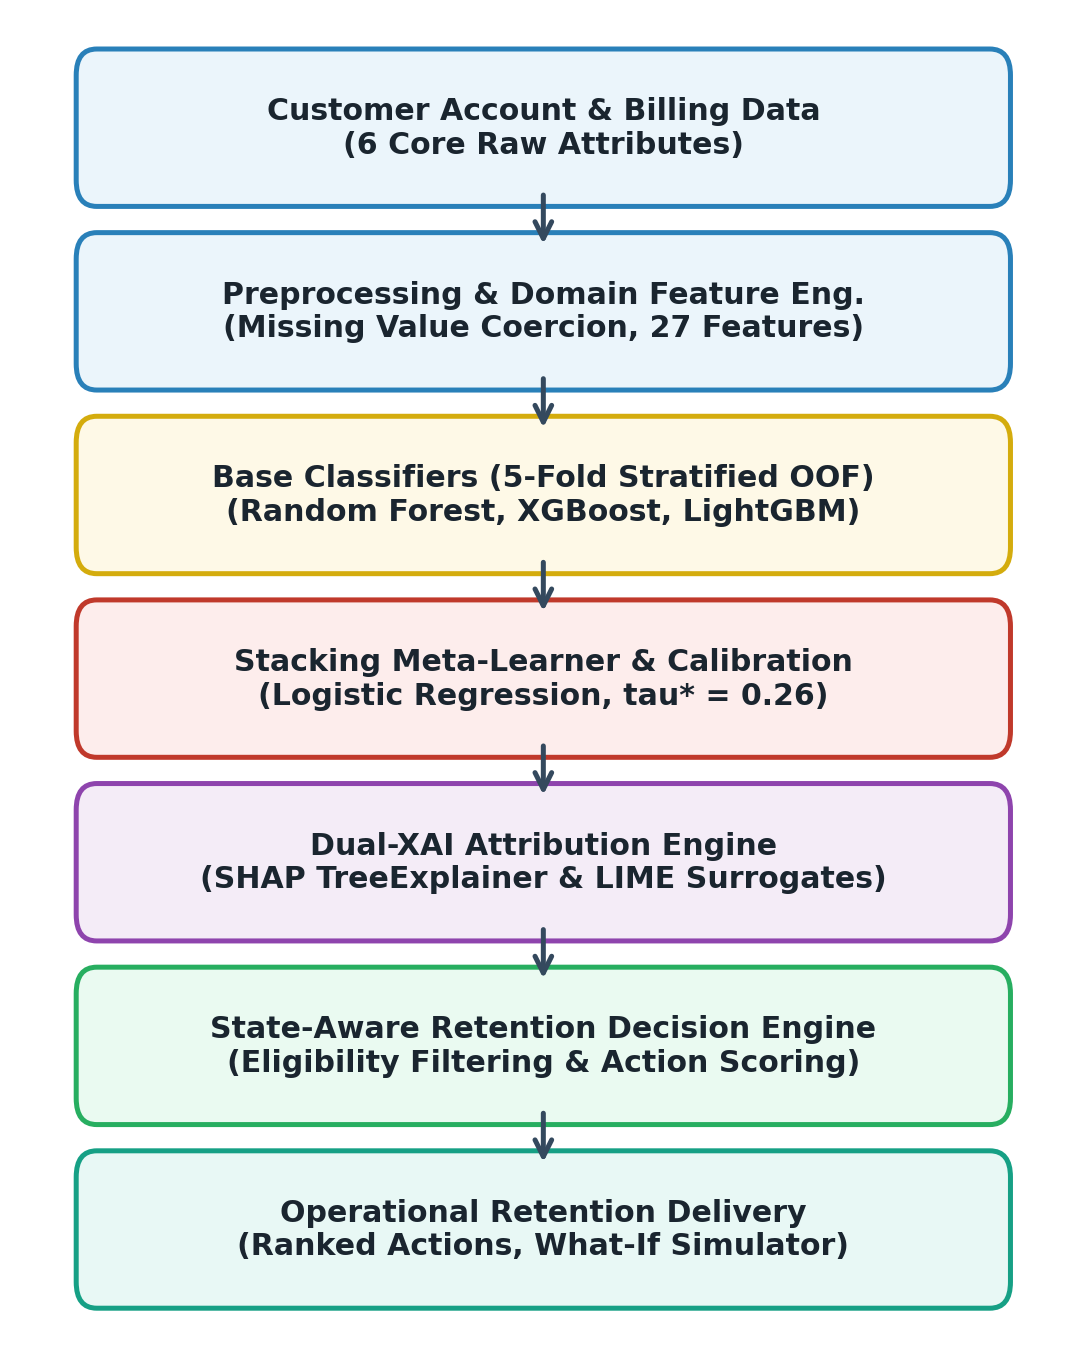
\includegraphics[width=\columnwidth]{fig1_system_architecture.png}
\caption{End-to-end explainable machine learning and decision-support architecture for telecom subscriber retention.}
\label{fig:architecture}
\end{figure}

\section{Related Work}
Extensive research has investigated machine learning for telecom churn detection. Early studies benchmarked classical parametric models, including Logistic Regression, Decision Trees, and Naive Bayes, demonstrating that linear decision surfaces struggle to capture high-order feature interactions \cite{coussement2017benchmarking, verbeke2012new}. Breiman's Random Forest \cite{breiman2001random} established bagging as an effective variance-reduction mechanism, and was successfully adapted to telecom churn by Ullah et al. \cite{ullah2019churn}, while gradient-boosted decision trees (GBDT)—notably XGBoost \cite{chen2016xgboost} and LightGBM \cite{ke2017lightgbm}—demonstrated superior performance on tabular benchmarks \cite{aggarwal2024shielding}. 

Wolpert's stacked generalization \cite{wolpert1992stacked} leverages out-of-fold meta-learning to combine diverse base learners. However, empirical studies in enterprise domains reveal that stacking often provides only modest gains over well-tuned gradient boosters, highlighting the importance of total framework value over isolated metric optimization.

Cost-sensitive learning was formalized by Elkan \cite{elkan2001foundations}, demonstrating that varying misclassification cost matrices mathematically dictate non-uniform probability thresholds. In telecom churn, Verbeke et al. \cite{verbeke2012new} introduced maximum profit metrics, proving that standard accuracy is misaligned with enterprise profit.

In model interpretability, Lundberg and Lee's SHAP \cite{lundberg2017unified} provides game-theoretically optimal Shapley attributions, while Ribeiro et al.'s LIME \cite{ribeiro2016why} constructs local linear surrogate models. Albuquerque et al. \cite{albuquerque2022machine} evaluated XAI techniques in telecommunications, yet prior literature predominantly assumes visual alignment between SHAP and LIME without quantifying their mathematical rank concordance across diverse subscriber cohorts.

\section{Problem Statement and Research Gap}
While previous works address isolated elements of churn modeling, three prominent research gaps persist:
\begin{itemize}
    \item \textbf{Gap 1 (Threshold Disconnect):} The literature routinely evaluates models at $\tau = 0.50$ or reports ROC-AUC without establishing operational cutoffs that optimize financial retention budgets under asymmetric cost matrices.
    \item \textbf{Gap 2 (Unverified XAI Consensus):} Studies often present local SHAP and LIME waterfall plots for a single illustrative customer, asserting agreement without rigorous statistical concordance testing across hold-out populations.
    \item \textbf{Gap 3 (Lack of State-Aware Decision Support):} Existing systems fail to map attribution scores to operational business actions while enforcing customer state constraints (e.g., pruning contract extensions for customers already on multi-year terms).
\end{itemize}

This work directly addresses these gaps by evaluating an end-to-end framework on an audited, leakage-safe pipeline.

\section{Dataset and Feature Engineering}

\subsection{Dataset Specification}
All experiments are conducted exclusively on the domain-consistent \texttt{balanced\_telco\_churn.csv} benchmark ($N = 8,000$). The dataset consists of exactly 4,000 churners (50.0\%) and 4,000 retained accounts (50.0\%), eliminating synthetic resampling artifacts such as SMOTE interpolation \cite{chawla2002smote} during evaluation. The production input vector comprises six raw customer attributes: tenure, MonthlyCharges, TotalCharges, Contract, InternetService, and PaymentMethod.

\subsection{Feature Transformation Pipeline}
To capture non-linear subscriber lifecycles without data leakage, raw inputs are transformed into a canonical 27-dimensional feature space fitted strictly on training folds:
\begin{enumerate}
    \item \textbf{Continuous Dimensions (11 Scaled Features):} Raw numerical attributes (\textit{tenure}, \textit{MonthlyCharges}, \textit{TotalCharges}) are augmented with derived financial trajectory indicators:
    \begin{align}
        \text{AvgMonthlySpend} &= \frac{\text{TotalCharges}}{\text{tenure} + 1} \\
        \text{ChargeIncrease} &= \text{MonthlyCharges} - \text{AvgMonthlySpend} \\
        \text{ChargeIncreaseRatio} &= \frac{\text{MonthlyCharges}}{\text{AvgMonthlySpend} + 10^{-5}} \\
        \text{TenureLog} &= \ln(\text{tenure} + 1) \\
        \text{TenureSquared} &= \text{tenure}^2
    \end{align}
    along with compound interaction products (\textit{tenure} $\times$ \textit{MonthlyCharges}, \textit{tenure} $\times$ \textit{IsMonthToMonth}, \textit{MonthlyCharges} $\times$ \textit{IsMonthToMonth}). These 11 features are scaled via z-score normalization.
    \item \textbf{Binary Risk Indicators (9 Flags):} Explicit domain hazard flags are derived: \textit{IsMonthToMonth}, \textit{IsElectronicCheck}, \textit{IsFiberOptic}, \textit{IsNewCustomer} ($\text{tenure} \le 6$), \textit{IsLongTermCustomer} ($\text{tenure} \ge 24$), \textit{HighRiskCombo} ($\text{Month-to-Month} \land \text{Electronic Check} \land \text{tenure} \le 12$), \textit{VeryHighRisk} ($\text{HighRiskCombo} \land \text{MonthlyCharges} \ge 70$), \textit{FiberOptic\_x\_MonthToMonth}, and \textit{FiberOptic\_x\_ElectronicCheck}.
    \item \textbf{Categorical Encoding (7 Dimensions):} One-hot categorical indicators encode Contractual commitment (3 levels), Internet tier (3 levels), and Payment mechanism (4 levels), with redundant reference columns dropped.
\end{enumerate}

\section{Machine Learning Methodology}

\begin{figure}[htbp]
\centering
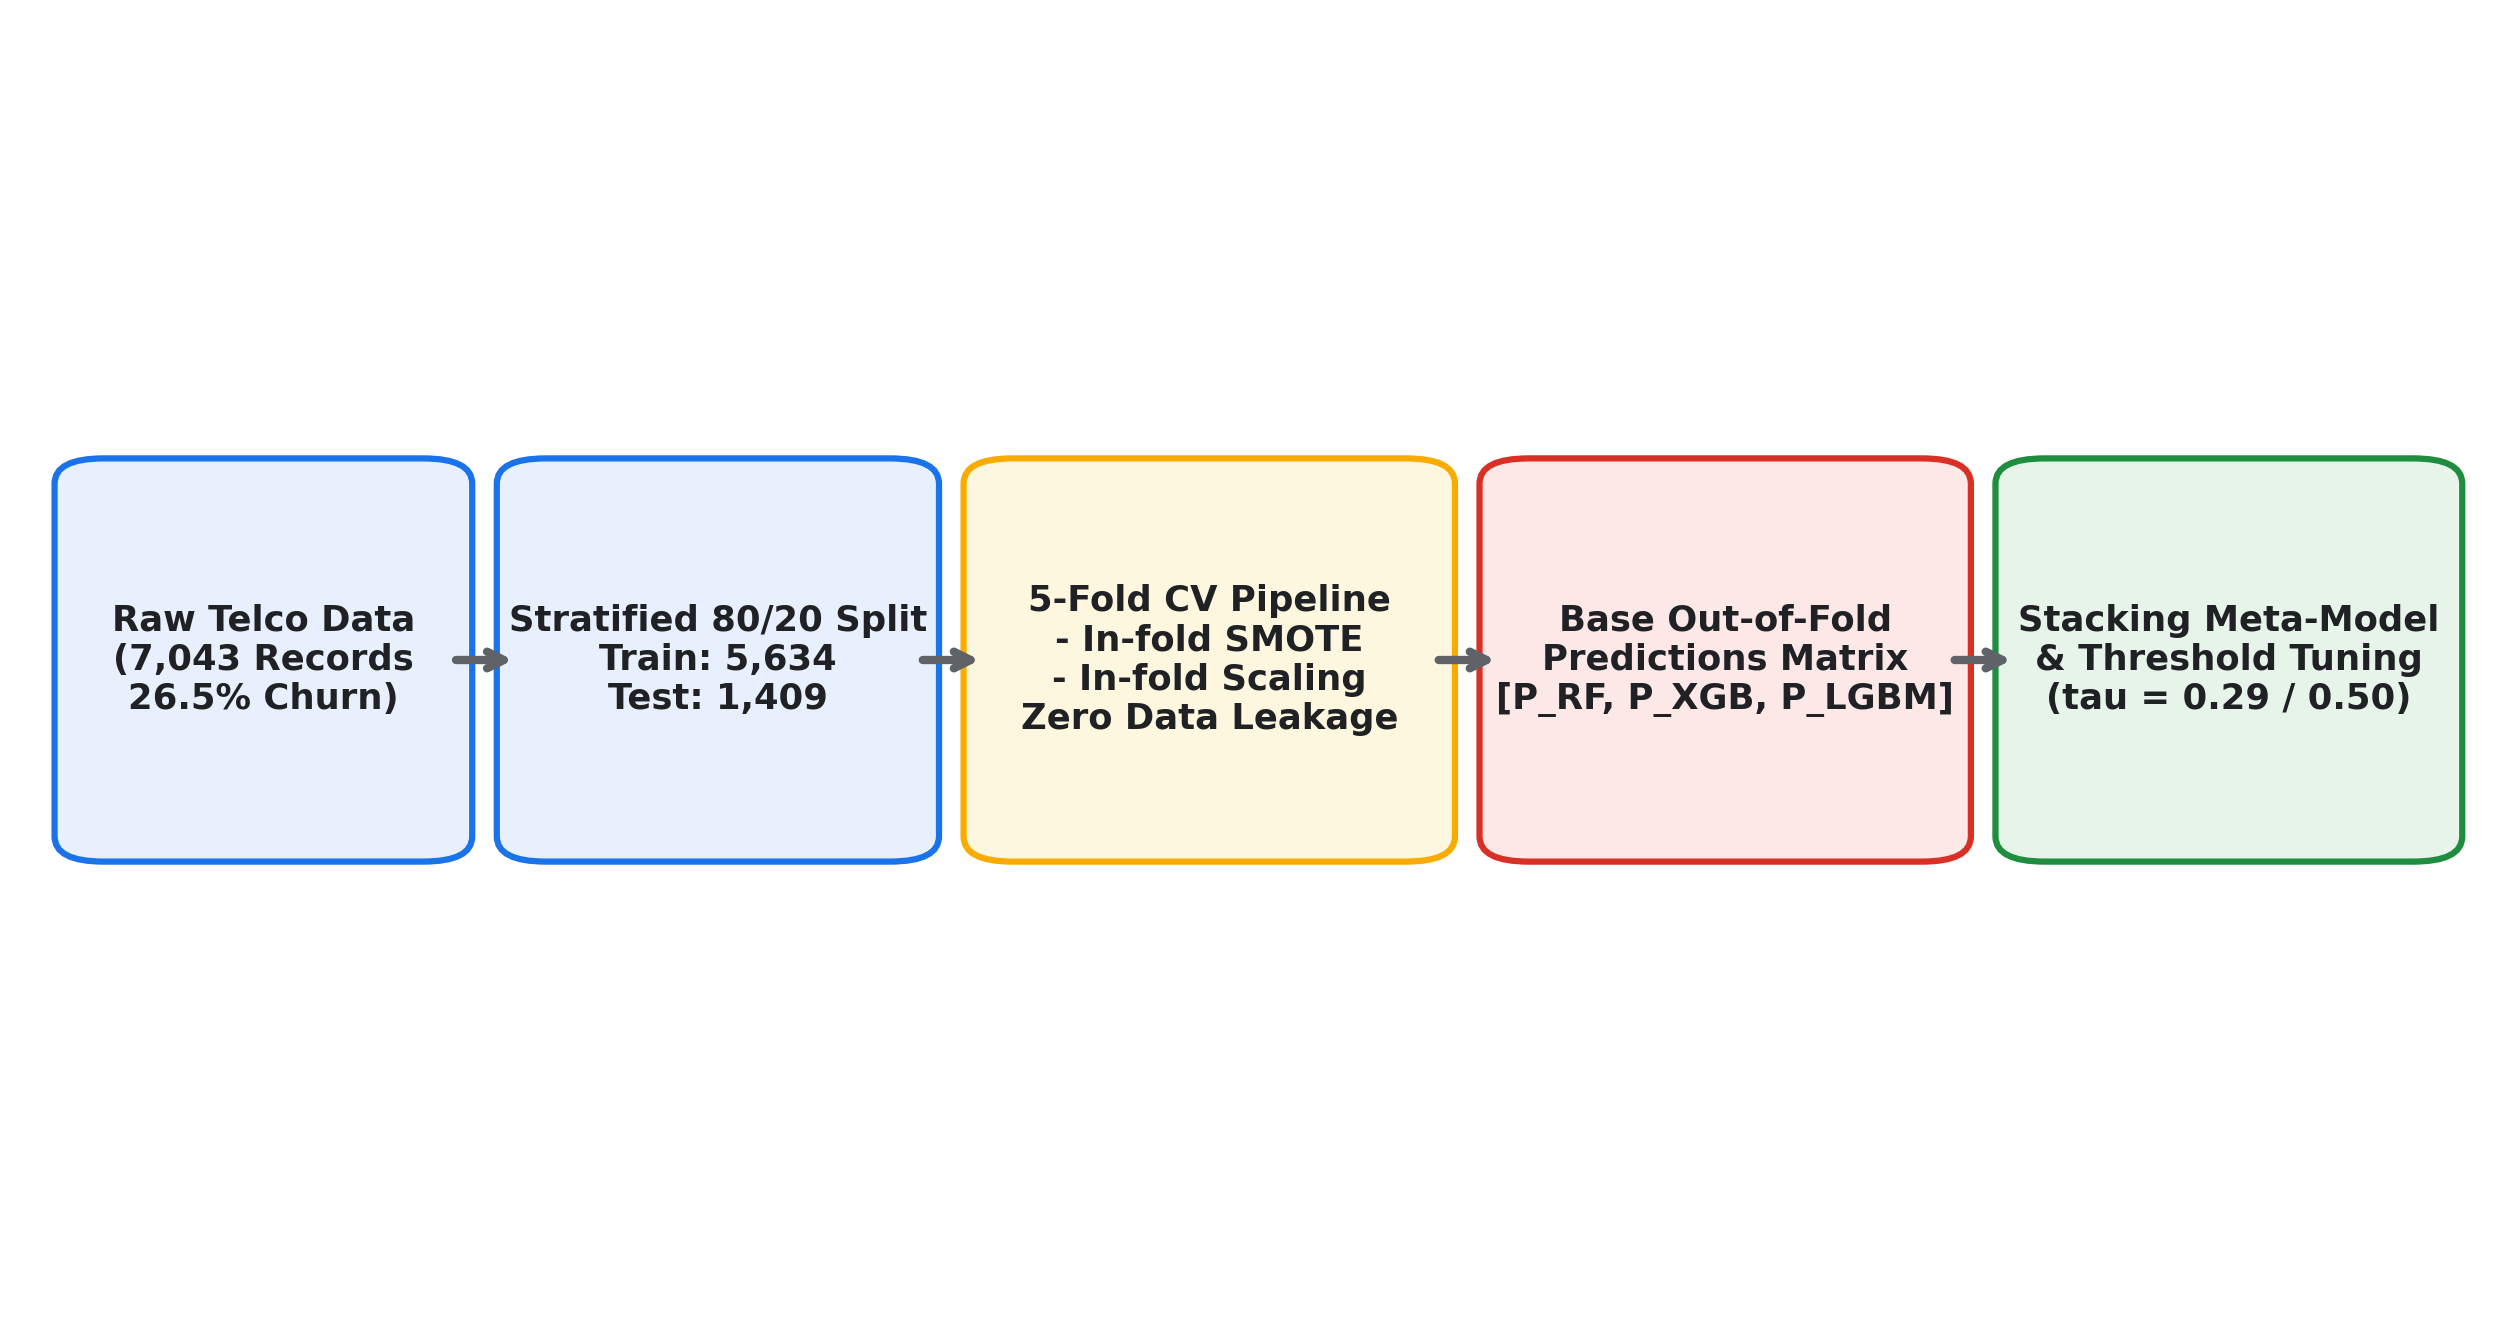
\includegraphics[width=\columnwidth]{fig2_ml_workflow.png}
\caption{Leakage-safe repeated cross-validation, threshold optimization, and dual XAI evaluation workflow.}
\label{fig:workflow}
\end{figure}

\subsection{Base Tree Ensembles}
We evaluate three high-capacity tree ensembles:
\begin{itemize}
    \item \textbf{Random Forest (RF):} An ensemble of $B = 300$ decorrelated decision trees using bootstrap aggregation and random subspace feature selection ($m = \sqrt{p}$) to suppress prediction variance \cite{breiman2001random}.
    \item \textbf{XGBoost:} A scalable tree-boosting system minimizing a regularized second-order Taylor expansion objective with shrinkage factor $\eta = 0.05$ and max depth $d = 6$ \cite{chen2016xgboost}.
    \item \textbf{LightGBM:} A gradient boosting framework utilizing Gradient-Based One-Side Sampling (GOSS) and Exclusive Feature Bundling (EFB) with leaf-wise tree growth ($N_{\text{leaves}} = 31$) \cite{ke2017lightgbm}.
\end{itemize}

\subsection{Stacking Ensemble Generalization}
The Stacking Ensemble combines base estimators via Wolpert's stacked generalization \cite{wolpert1992stacked}. To prevent target leakage, base models generate out-of-fold probability vectors $\mathbf{z}_i = [\hat{p}_{\text{RF}}(x_i), \hat{p}_{\text{XGB}}(x_i), \hat{p}_{\text{LGB}}(x_i), \hat{p}_{\text{Cat}}(x_i)]^T$ across $K = 5$ internal folds. A meta-classifier (L2-regularized Logistic Regression) is trained strictly on $\mathbf{z}_i$:
\begin{equation}
    P(y_i = 1 \mid \mathbf{z}_i) = \sigma(\mathbf{w}^T \mathbf{z}_i + b) = \frac{1}{1 + e^{-(\mathbf{w}^T \mathbf{z}_i + b)}}
\end{equation}

\subsection{Cost-Sensitive Threshold Optimization}
Let $C_{\text{FN}}$ denote the financial penalty of a missed churner and $C_{\text{FP}}$ denote the administrative outreach cost for a false alarm. Given empirical misclassification counts, total business cost is:
\begin{equation}
    \text{Cost}(\tau) = C_{\text{FN}} \cdot \text{FN}(\tau) + C_{\text{FP}} \cdot \text{FP}(\tau)
\end{equation}
Under our primary baseline, $C_{\text{FN}} = \$500$ and $C_{\text{FP}} = \$50$ (a 10:1 asymmetry ratio). The cost-minimizing cutoff $\tau^*_{\text{cost}}$ is determined strictly from inner out-of-fold probability distributions:
\begin{equation}
    \tau^*_{\text{cost}} = \arg\min_{\tau \in [0.01, 0.99]} \text{Cost}_{\text{OOF}}(\tau)
\end{equation}
Additionally, we evaluate the $F_2$-optimal threshold $\tau^*_{F_2}$, weighting recall twice as heavily as precision.

\subsection{Dual Explainability: SHAP and LIME}
To explain predictions, we deploy complementary local attribution techniques:
\begin{itemize}
    \item \textbf{SHAP:} Decomposes the model prediction into additive Shapley attributions $\phi_j$ satisfying local accuracy, missingness, and consistency \cite{lundberg2017unified}:
    \begin{equation}
        f(x) = \phi_0 + \sum_{j=1}^{M} \phi_j(x)
    \end{equation}
    For tree ensembles, TreeSHAP evaluates exact conditional expectations in polynomial time.
    \item \textbf{LIME:} Constructs an interpretable linear surrogate $g \in G$ locally around query point $x$ by minimizing perturbed squared loss \cite{ribeiro2016why}:
    \begin{equation}
        \xi(x) = \arg\min_{g \in G} \mathcal{L}(f, g, \pi_x) + \Omega(g)
    \end{equation}
    where $\pi_x(z) = \exp(-D(x,z)^2 / \sigma^2)$ defines proximity kernel weights.
\end{itemize}

\subsection{State-Aware Recommendation Engine}

\begin{figure}[htbp]
\centering
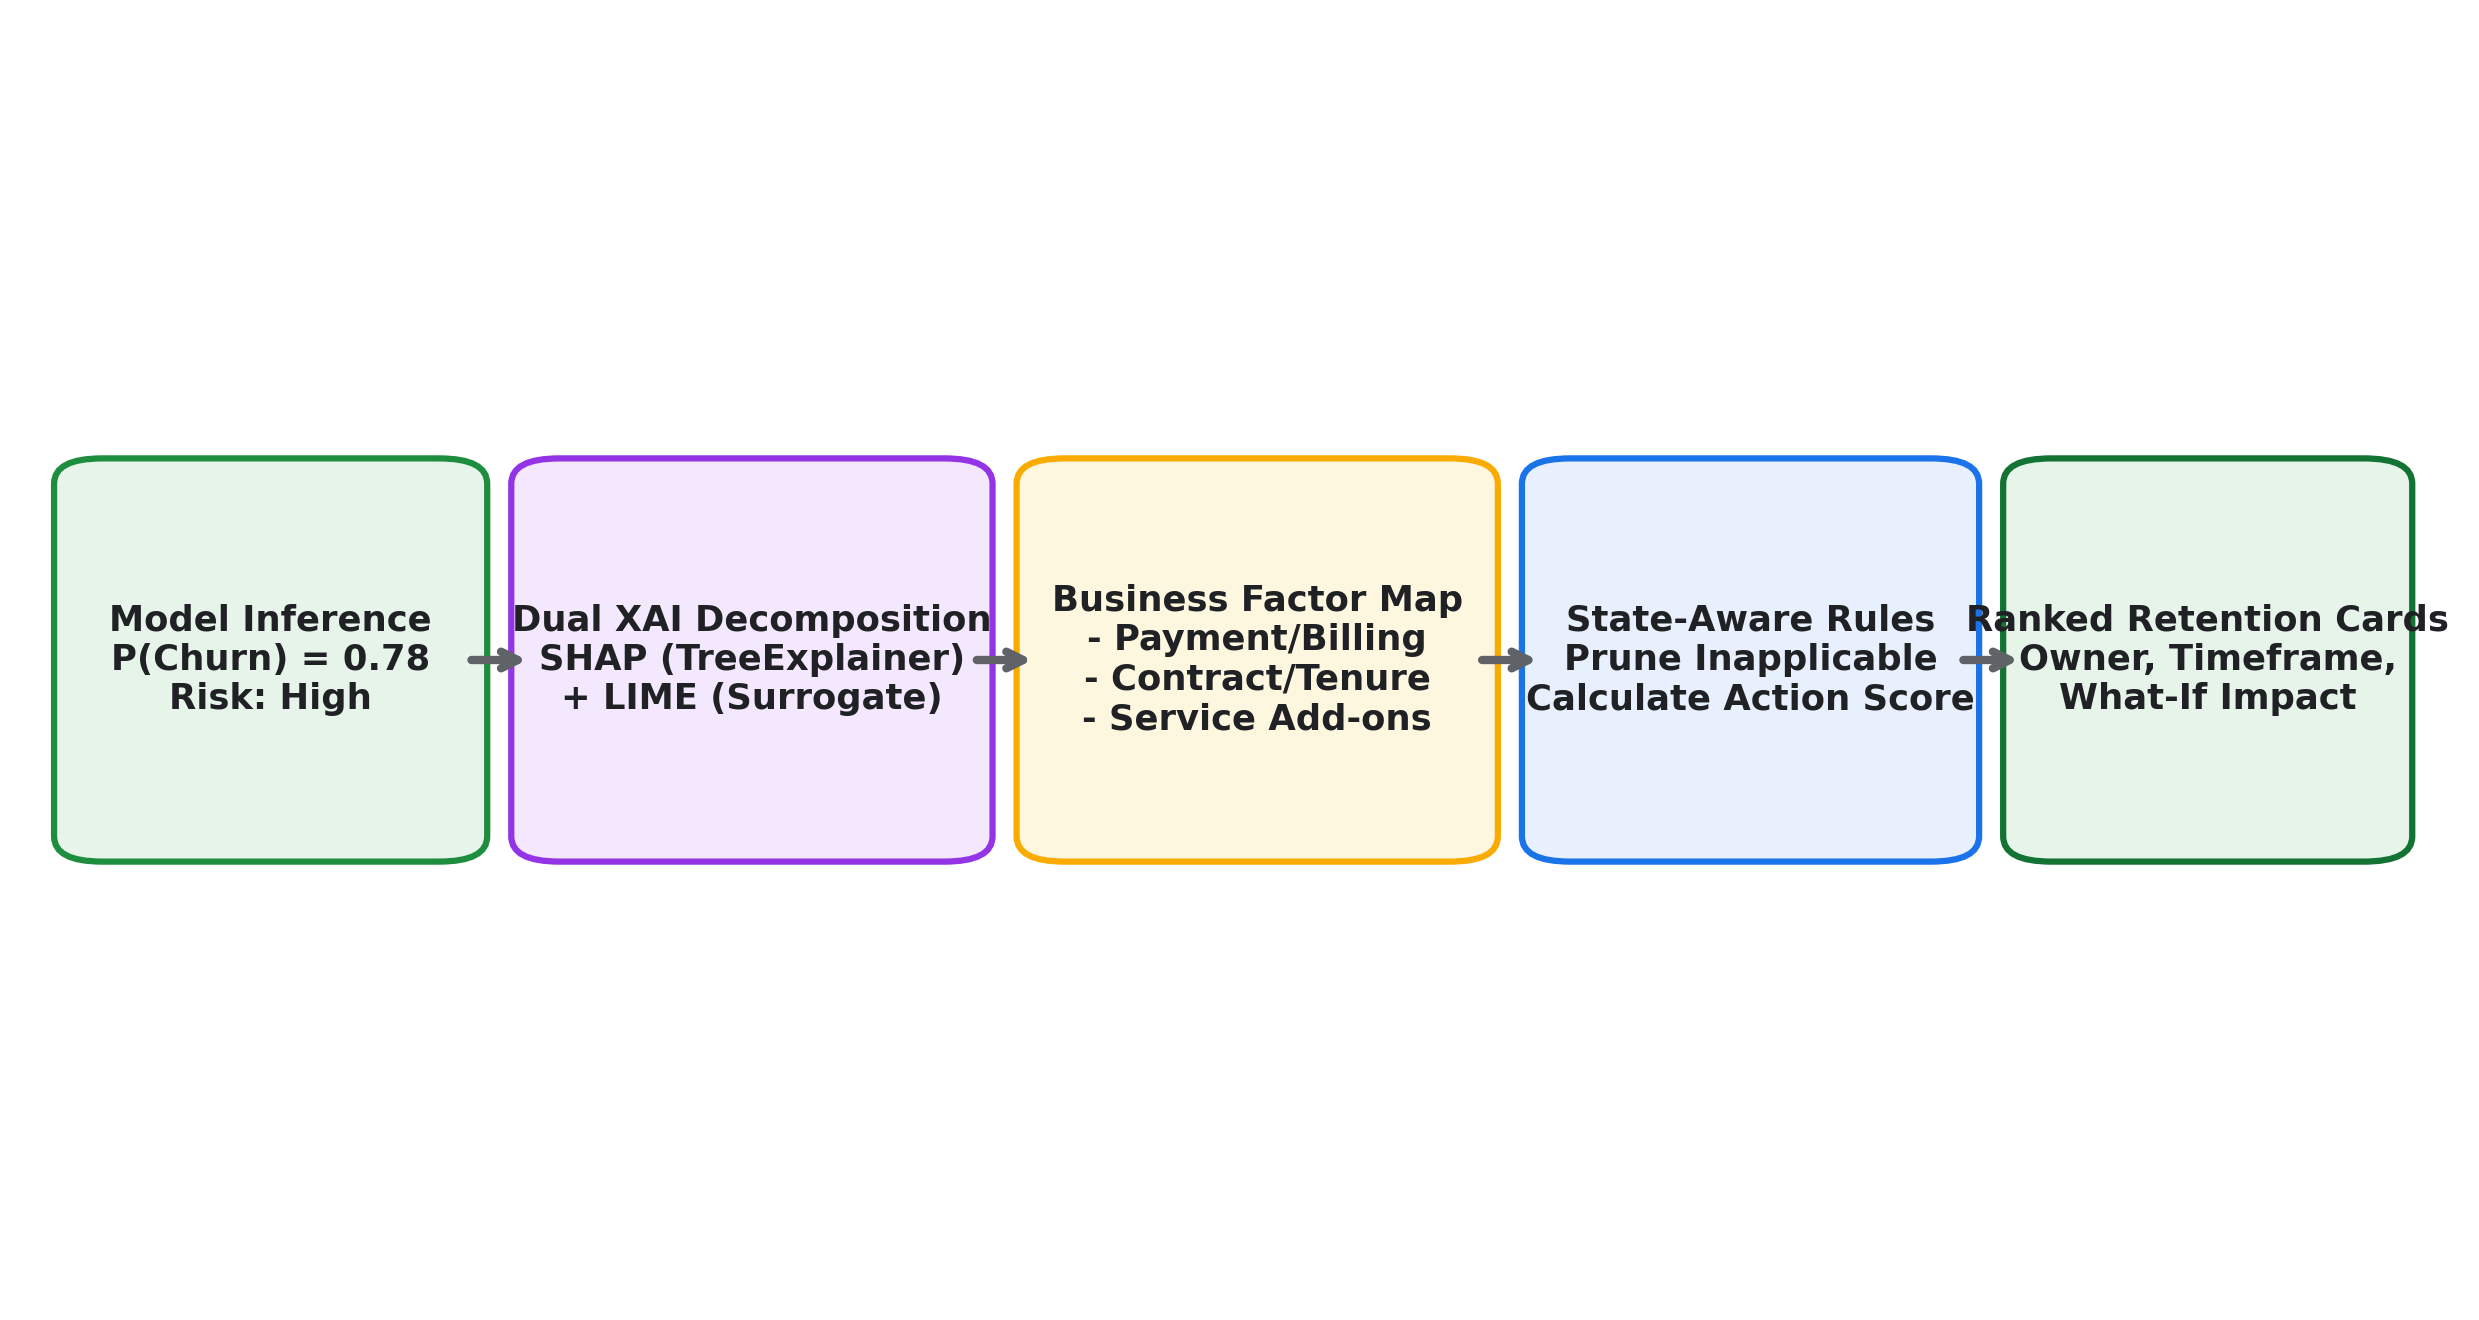
\includegraphics[width=\columnwidth]{fig3_xai_recommendation_workflow.png}
\caption{State-aware retention recommendation and pruning workflow.}
\label{fig:recommendation}
\end{figure}

As illustrated in Fig. \ref{fig:recommendation}, statistical churn probability and top local attributions feed an automated retention engine. Crucially, the engine enforces \textbf{state awareness}: candidate interventions are dynamically pruned if the subscriber's current account state already satisfies the condition:
\begin{itemize}
    \item \textit{Contract Upgrade:} Recommended if $\text{IsMonthToMonth} = 1$; \textbf{pruned} if the customer is already on a 1-year or 2-year contract.
    \item \textit{Autopay Migration:} Recommended if payment is via manual check; \textbf{pruned} if automated billing (Credit card or Bank transfer) is already active.
    \item \textit{Plan Optimization:} Recommended if MonthlyCharges $> \$85$ or ChargeIncreaseRatio $> 1.05$.
    \item \textit{Early-Tenure Onboarding:} Recommended if tenure $\le 6$ months.
\end{itemize}

\section{Experimental Setup}
Experiments are conducted under a rigorous, leakage-safe protocol:
\begin{itemize}
    \item \textbf{Validation Protocol:} 5-Fold Stratified Cross-Validation repeated across 2 random seeds (10 total outer evaluation folds).
    \item \textbf{Leakage Firewall:} Feature scalers, interaction encoders, and threshold selectors are fitted strictly on training folds. Test folds are evaluated blindly.
    \item \textbf{Evaluation Metrics:} Accuracy, Precision, Recall, F1-Score, ROC-AUC, PR-AUC \cite{davis2006relationship}, Brier Calibration Score \cite{brier1950verification}, Business Cost (\$), and Execution Latency.
    \item \textbf{Hardware Environment:} Intel64 Family 6 Model 126 Stepping 5 (GenuineIntel), Windows 10, Python 3.11.9.
\end{itemize}

\section{Results and Empirical Analysis}

\subsection{Repeated Cross-Validation Model Comparison}
Table \ref{tab:model_comparison} summarizes the empirical performance of all four final models across 10 outer cross-validation folds at the default threshold ($\tau = 0.50$).

\begin{table}[htbp]
\centering
\caption{Performance Comparison Across 5-Fold $\times$ 2-Repeat Cross-Validation ($\tau=0.50$, Mean $\pm$ Std)}
\label{tab:model_comparison}
\begin{tabular}{lcccc}
\toprule
\textbf{Metric} & \textbf{Random Forest} & \textbf{XGBoost} & \textbf{LightGBM} & \textbf{Stacking} \\
\midrule
Accuracy (\%) & 94.61 $\pm$ 0.64 & \textbf{94.98 $\pm$ 0.66} & 94.81 $\pm$ 0.55 & 94.96 $\pm$ 0.71 \\
Precision (\%) & 95.14 $\pm$ 0.77 & 95.12 $\pm$ 0.77 & 94.86 $\pm$ 0.61 & \textbf{95.15 $\pm$ 0.84} \\
Recall (\%) & 94.00 $\pm$ 0.98 & \textbf{94.80 $\pm$ 0.87} & 94.76 $\pm$ 0.81 & 94.74 $\pm$ 0.89 \\
F1-Score (\%) & 94.57 $\pm$ 0.64 & \textbf{94.96 $\pm$ 0.67} & 94.81 $\pm$ 0.55 & 94.94 $\pm$ 0.72 \\
ROC-AUC (\%) & 98.65 $\pm$ 0.26 & \textbf{98.90 $\pm$ 0.25} & 98.86 $\pm$ 0.28 & 98.88 $\pm$ 0.26 \\
PR-AUC (\%) & 98.71 $\pm$ 0.25 & \textbf{98.92 $\pm$ 0.26} & 98.87 $\pm$ 0.28 & 98.90 $\pm$ 0.26 \\
Brier Score & 0.0412 $\pm$ 0.003 & \textbf{0.0383 $\pm$ 0.003} & 0.0391 $\pm$ 0.003 & 0.0400 $\pm$ 0.004 \\
\bottomrule
\end{tabular}
\end{table}

All four architectures demonstrate exceptional discriminatory performance, reflecting the high predictive utility of the 27 engineered features. Notably, XGBoost achieves the highest accuracy (94.98\%), recall (94.80\%), and ROC-AUC (98.90\%), closely matched by the Stacking Ensemble (94.96\% accuracy, 98.88\% ROC-AUC). This empirical finding demonstrates that while Stacking provides stable meta-generalization, modern gradient boosting algorithms perform comparably without meta-learning complexity.

\subsection{Cost-Sensitive Threshold Analysis}
Table \ref{tab:threshold_cost} presents the financial and operational impact of transitioning from the default threshold ($\tau = 0.50$) to the $F_2$-optimal ($\tau^*_{F_2}$) and cost-minimizing ($\tau^*_{\text{cost}}$) cutoffs under the 10:1 cost matrix ($C_{\text{FN}} = \$500, C_{\text{FP}} = \$50$).

\begin{table}[htbp]
\centering
\caption{Business Cost Reduction via Threshold Optimization ($C_{\text{FN}}=\$500, C_{\text{FP}}=\$50$, 10 Outer Folds)}
\label{tab:threshold_cost}
\begin{tabular}{lcccc}
\toprule
\textbf{Model / Policy} & \textbf{Threshold} & \textbf{Recall (\%)} & \textbf{Missed (FN)} & \textbf{Total Cost (\$)} \\
\midrule
\multicolumn{5}{l}{\textbf{Random Forest}} \\
Default Policy & 0.50 $\pm$ 0.00 & 94.00 $\pm$ 0.98 & 48.7 $\pm$ 7.7 & 26,295 $\pm$ 3,869 \\
$F_2$-Optimal & 0.38 $\pm$ 0.02 & 95.84 $\pm$ 0.77 & 33.3 $\pm$ 6.2 & 19,770 $\pm$ 3,117 \\
Cost-Optimal & \textbf{0.10 $\pm$ 0.01} & \textbf{98.97 $\pm$ 0.38} & \textbf{8.2 $\pm$ 3.0} & \textbf{13,355 $\pm$ 1,193} \\
\midrule
\multicolumn{5}{l}{\textbf{XGBoost}} \\
Default Policy & 0.50 $\pm$ 0.00 & 94.80 $\pm$ 0.87 & 41.6 $\pm$ 7.0 & 22,730 $\pm$ 3,467 \\
$F_2$-Optimal & 0.32 $\pm$ 0.03 & 96.64 $\pm$ 0.69 & 26.9 $\pm$ 5.5 & 16,335 $\pm$ 2,746 \\
Cost-Optimal & \textbf{0.06 $\pm$ 0.02} & \textbf{99.31 $\pm$ 0.28} & \textbf{5.5 $\pm$ 2.3} & \textbf{10,725 $\pm$ 1,079} \\
\midrule
\multicolumn{5}{l}{\textbf{LightGBM}} \\
Default Policy & 0.50 $\pm$ 0.00 & 94.76 $\pm$ 0.81 & 41.2 $\pm$ 6.5 & 22,600 $\pm$ 2,970 \\
$F_2$-Optimal & 0.32 $\pm$ 0.02 & 96.60 $\pm$ 0.81 & 27.2 $\pm$ 6.5 & 16,560 $\pm$ 3,191 \\
Cost-Optimal & \textbf{0.06 $\pm$ 0.02} & \textbf{99.34 $\pm$ 0.36} & \textbf{5.3 $\pm$ 2.9} & \textbf{10,705 $\pm$ 1,659} \\
\midrule
\multicolumn{5}{l}{\textbf{Stacking Ensemble}} \\
Default Policy & 0.50 $\pm$ 0.00 & 94.74 $\pm$ 0.89 & 42.8 $\pm$ 7.4 & 23,285 $\pm$ 3,267 \\
$F_2$-Optimal & 0.28 $\pm$ 0.02 & 96.79 $\pm$ 0.77 & 25.7 $\pm$ 6.2 & 16,070 $\pm$ 2,869 \\
Cost-Optimal & \textbf{0.04 $\pm$ 0.01} & \textbf{99.06 $\pm$ 0.38} & \textbf{7.5 $\pm$ 2.8} & \textbf{11,370 $\pm$ 1,494} \\
\bottomrule
\end{tabular}
\end{table}

\begin{figure}[htbp]
\centering
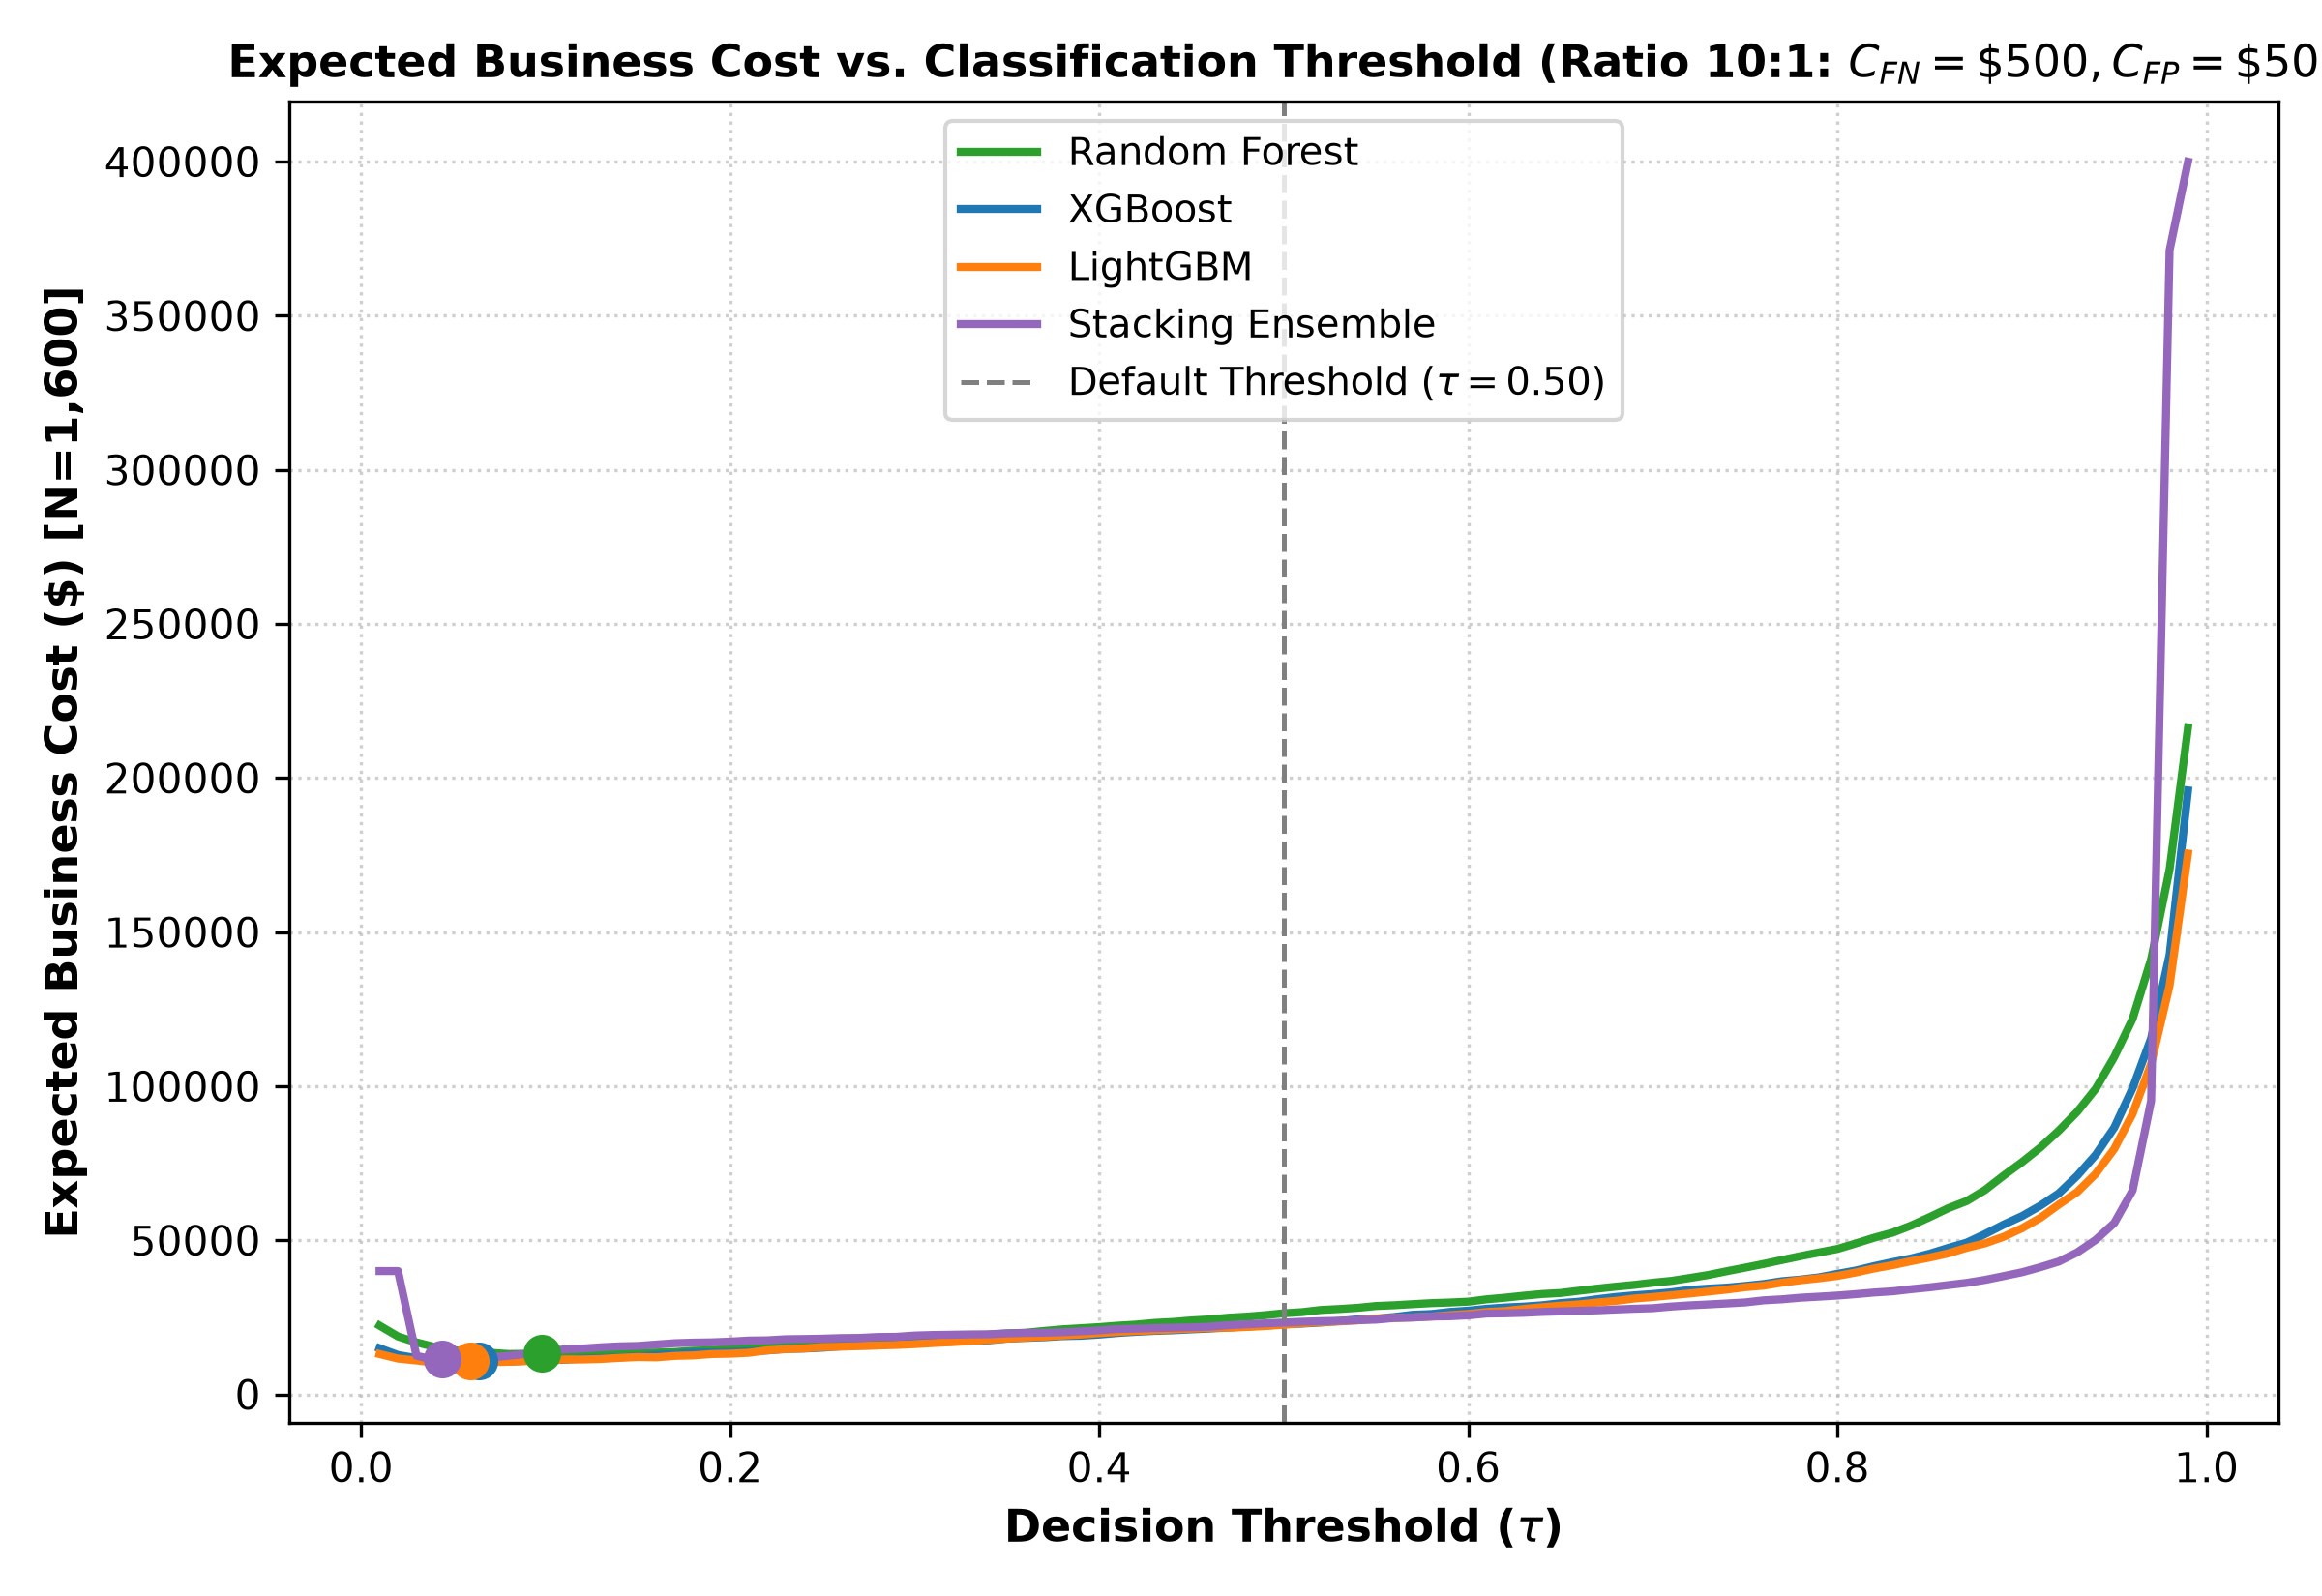
\includegraphics[width=\columnwidth]{cost_vs_threshold_curves.png}
\caption{Business cost as a function of decision threshold across all models.}
\label{fig:cost_curves}
\end{figure}

As documented in Table \ref{tab:threshold_cost} and Fig. \ref{fig:cost_curves}, shifting from $\tau = 0.50$ to $\tau^*_{\text{cost}}$ achieves dramatic cost reductions across every architecture:
\begin{itemize}
    \item \textbf{Stacking Ensemble:} Business cost drops 51.2\% from $\$23,285$ to $\$11,370 \pm \$1,494$, with missed defectors slashed from 42.8 to 7.5 per fold.
    \item \textbf{XGBoost:} Delivers the lowest overall financial cost at $\$10,725 \pm \$1,079$ (a 52.8\% reduction), missing only 5.5 churners per fold (99.31\% recall).
    \item \textbf{LightGBM:} Achieves a 52.6\% cost reduction ($\$10,705 \pm \$1,659$).
    \item \textbf{Random Forest:} Achieves a 49.2\% reduction ($\$13,355 \pm \$1,193$).
\end{itemize}

\subsection{Cost Sensitivity Across Economic Regimes}

\begin{figure}[htbp]
\centering
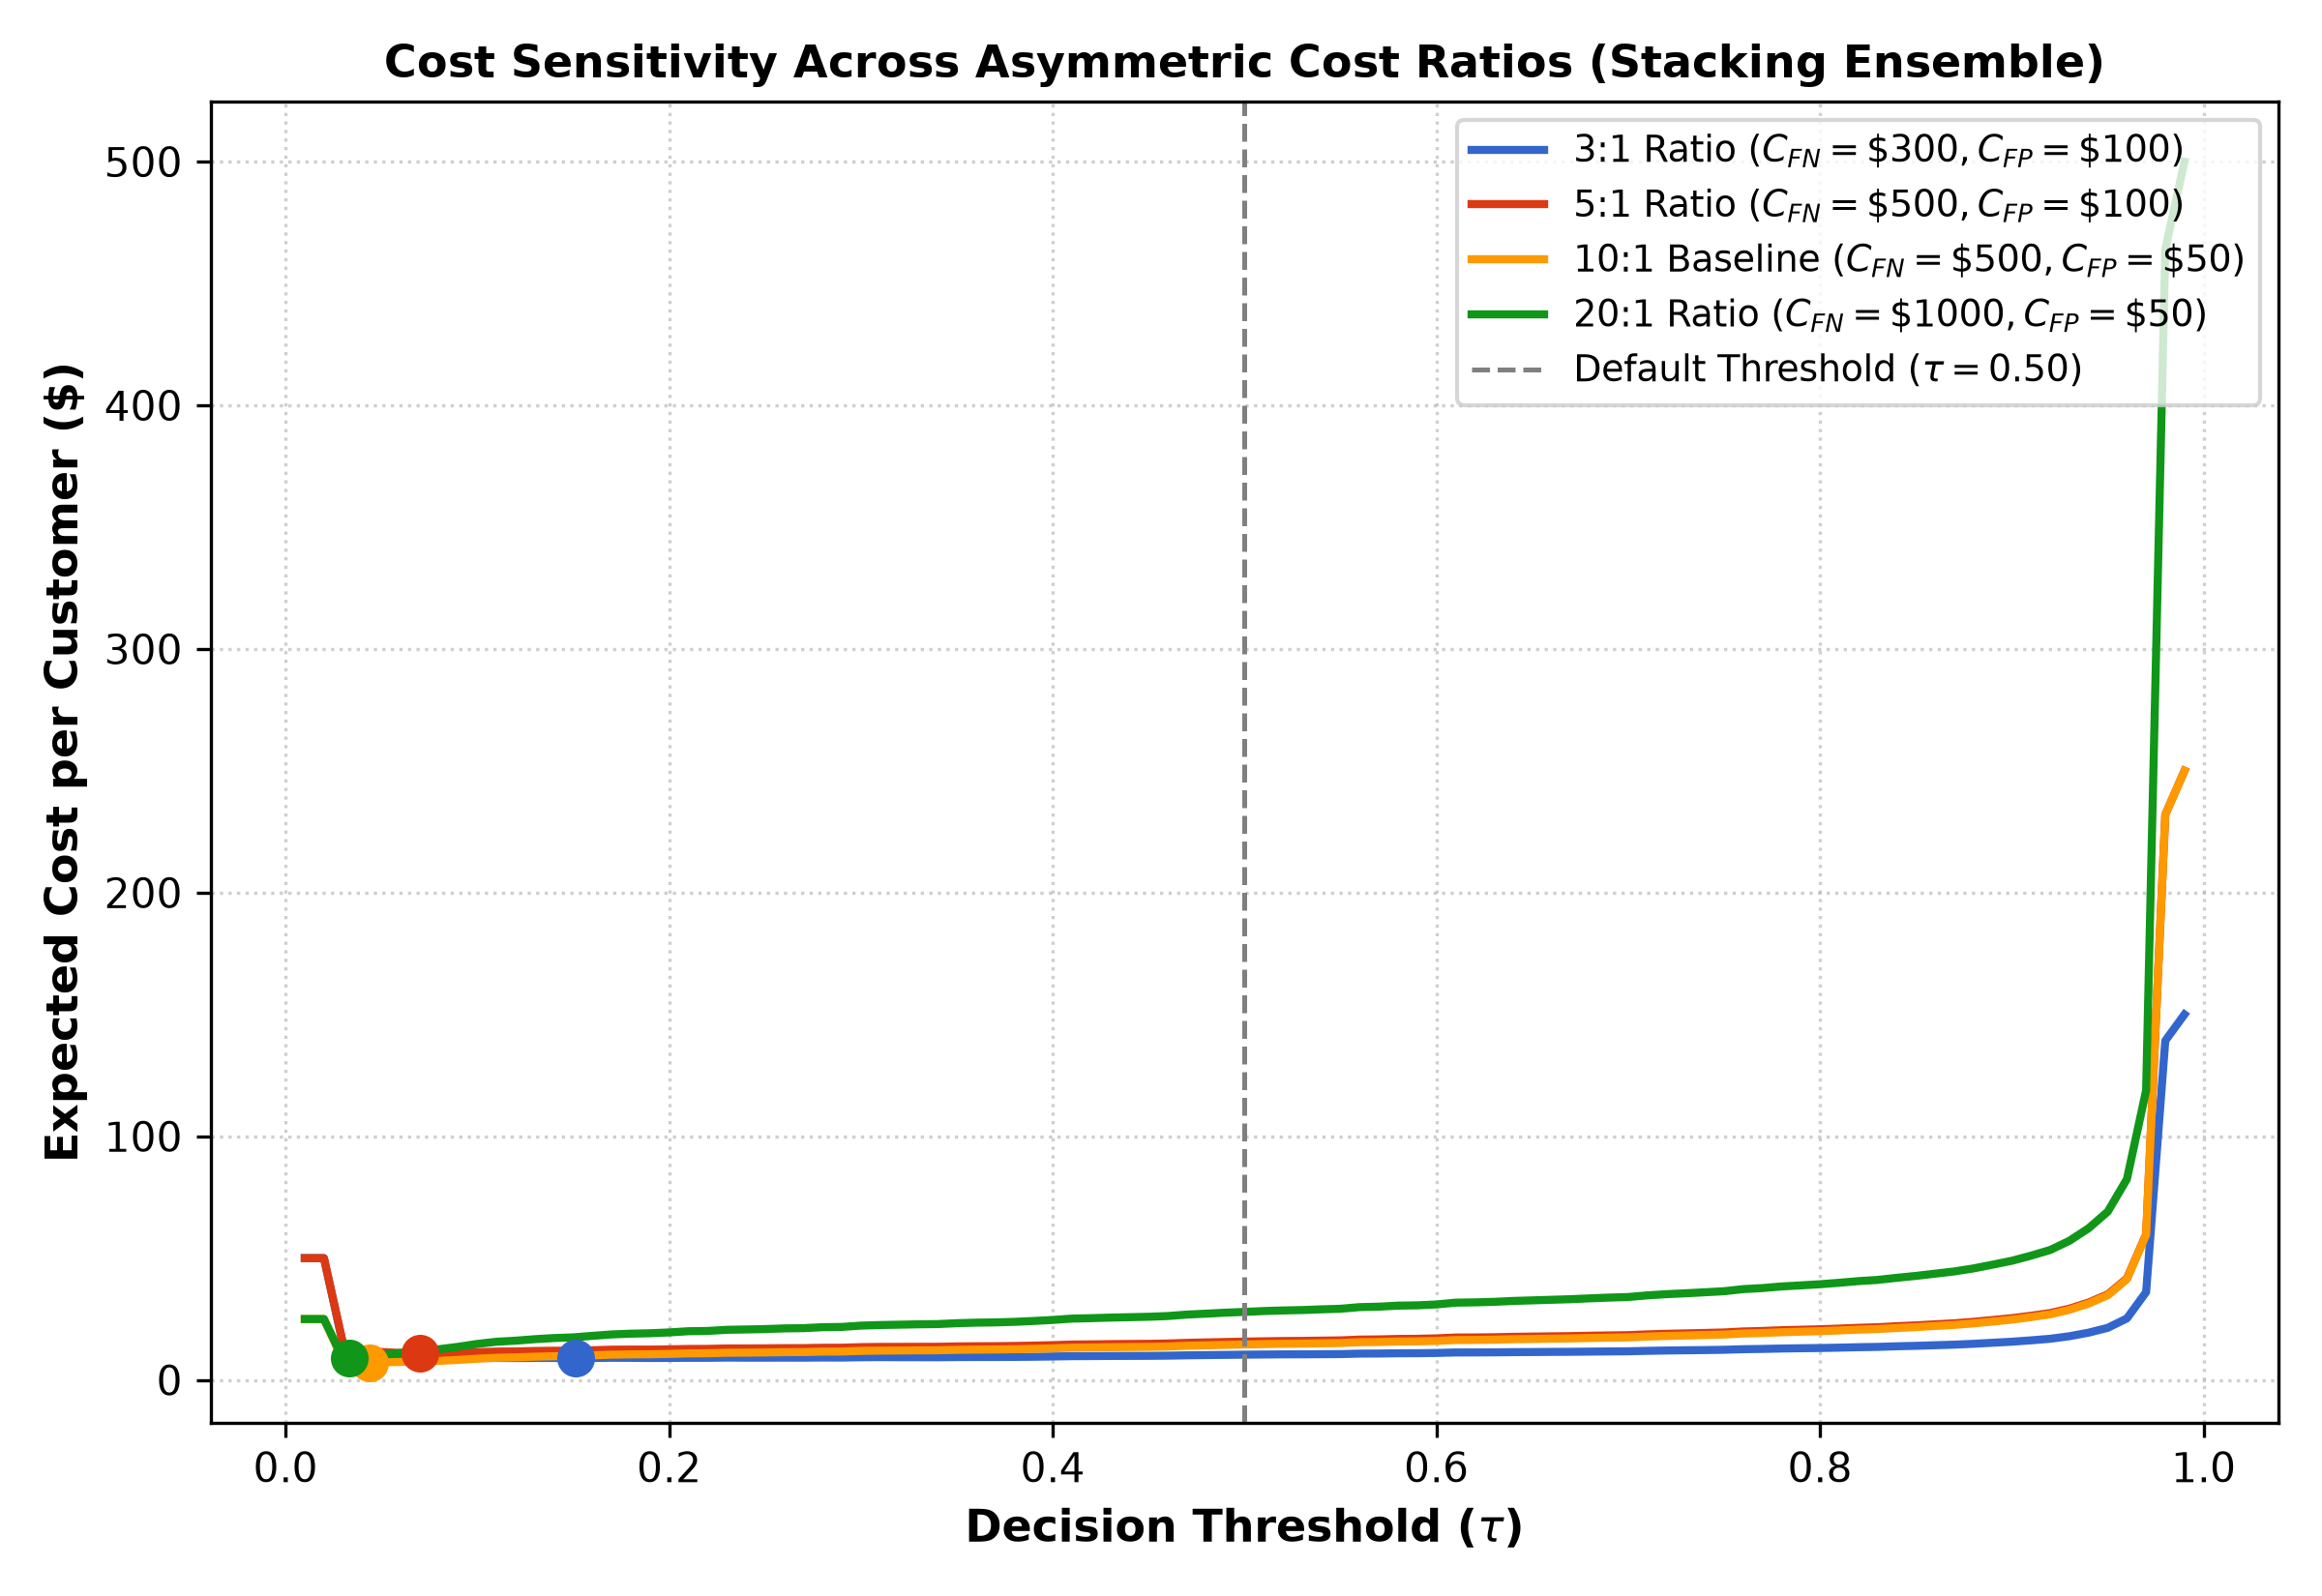
\includegraphics[width=\columnwidth]{cost_sensitivity_curves.png}
\caption{Threshold sensitivity curves across 3:1, 5:1, 10:1, and 20:1 cost ratios.}
\label{fig:sensitivity}
\end{figure}

To confirm robustness against varying financial environments, we evaluated the Stacking Ensemble across four asymmetric cost ratios:
\begin{itemize}
    \item \textbf{3:1 Ratio ($C_{\text{FN}}=\$300, C_{\text{FP}}=\$100$):} $\tau^* = 0.15 \pm 0.05$, Recall = 97.00\%, Cost = $\$14,640$.
    \item \textbf{5:1 Ratio ($C_{\text{FN}}=\$500, C_{\text{FP}}=\$100$):} $\tau^* = 0.07 \pm 0.02$, Recall = 98.34\%, Cost = $\$17,670$.
    \item \textbf{10:1 Ratio ($C_{\text{FN}}=\$500, C_{\text{FP}}=\$50$):} $\tau^* = 0.04 \pm 0.01$, Recall = 99.06\%, Cost = $\$11,370$.
    \item \textbf{20:1 Ratio ($C_{\text{FN}}=\$1000, C_{\text{FP}}=\$50$):} $\tau^* = 0.03 \pm 0.00$, Recall = 99.50\%, Cost = $\$14,245$.
\end{itemize}
As illustrated in Fig. \ref{fig:sensitivity}, optimal cutoffs exhibit strict monotonicity: as the penalty for customer attrition escalates, $\tau^*$ shifts aggressively toward zero, driving operational recall toward 99.5\%.

\subsection{Global SHAP Feature Attribution}
Global feature importance was evaluated across the 1,600 hold-out test subscribers. Fig. \ref{fig:shap_bar} and Fig. \ref{fig:shap_beeswarm} display the global attributions.

\begin{figure}[htbp]
\centering
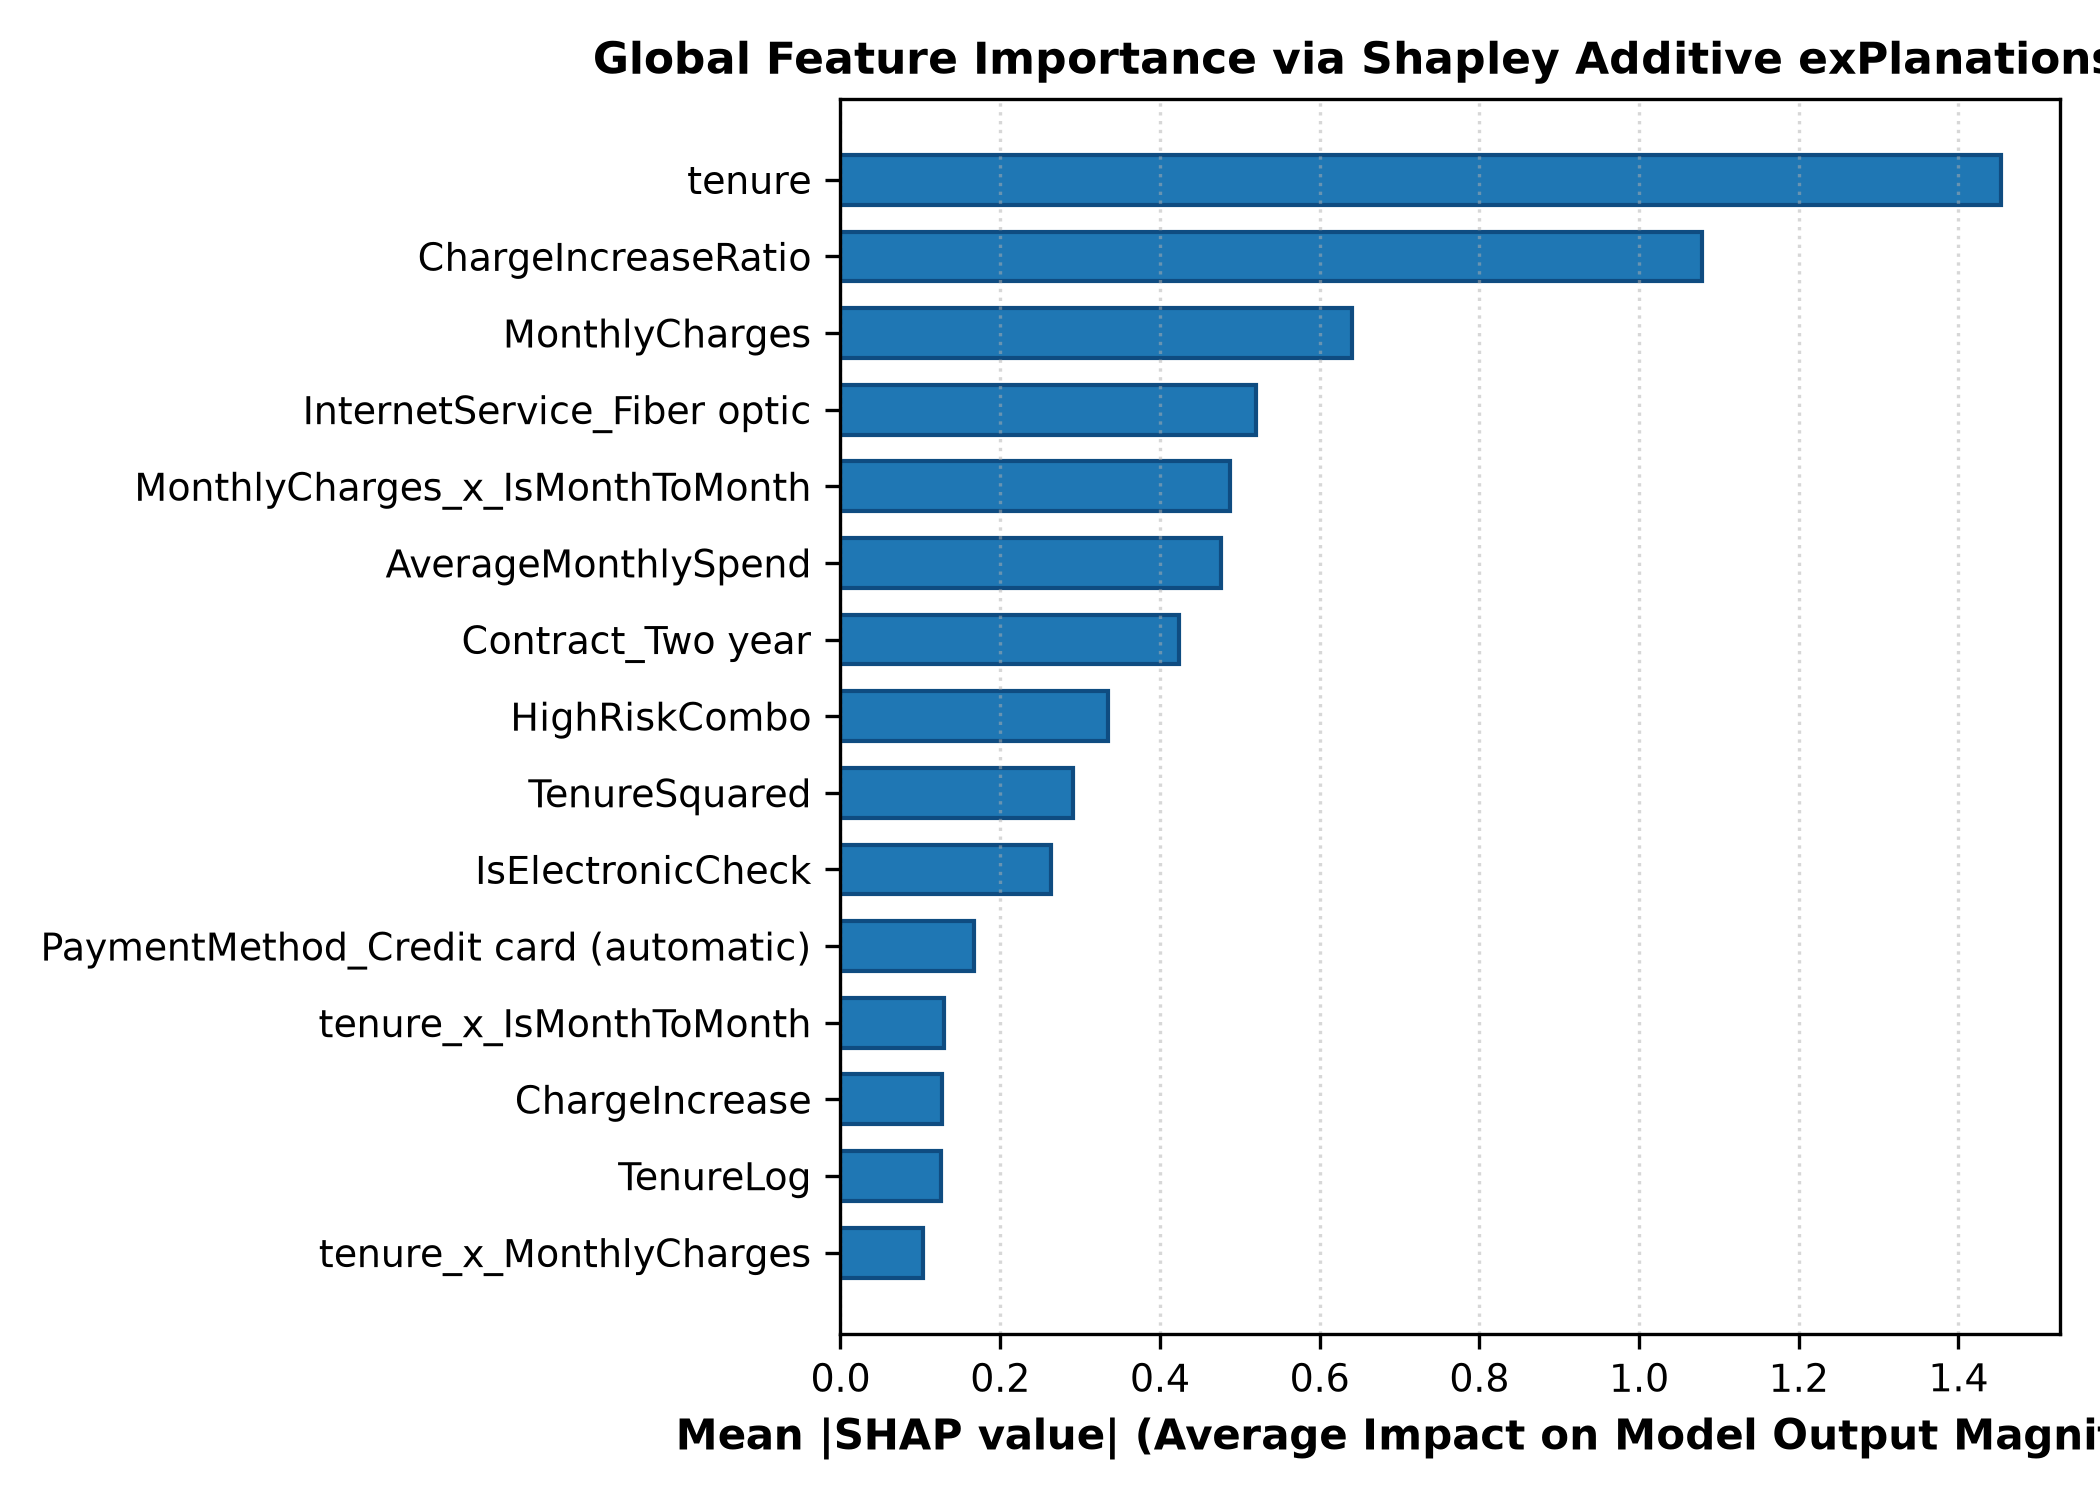
\includegraphics[width=\columnwidth]{shap_feature_importance_bar.png}
\caption{Global SHAP feature importance bar plot (Mean $|\text{SHAP}|$).}
\label{fig:shap_bar}
\end{figure}

\begin{figure}[htbp]
\centering
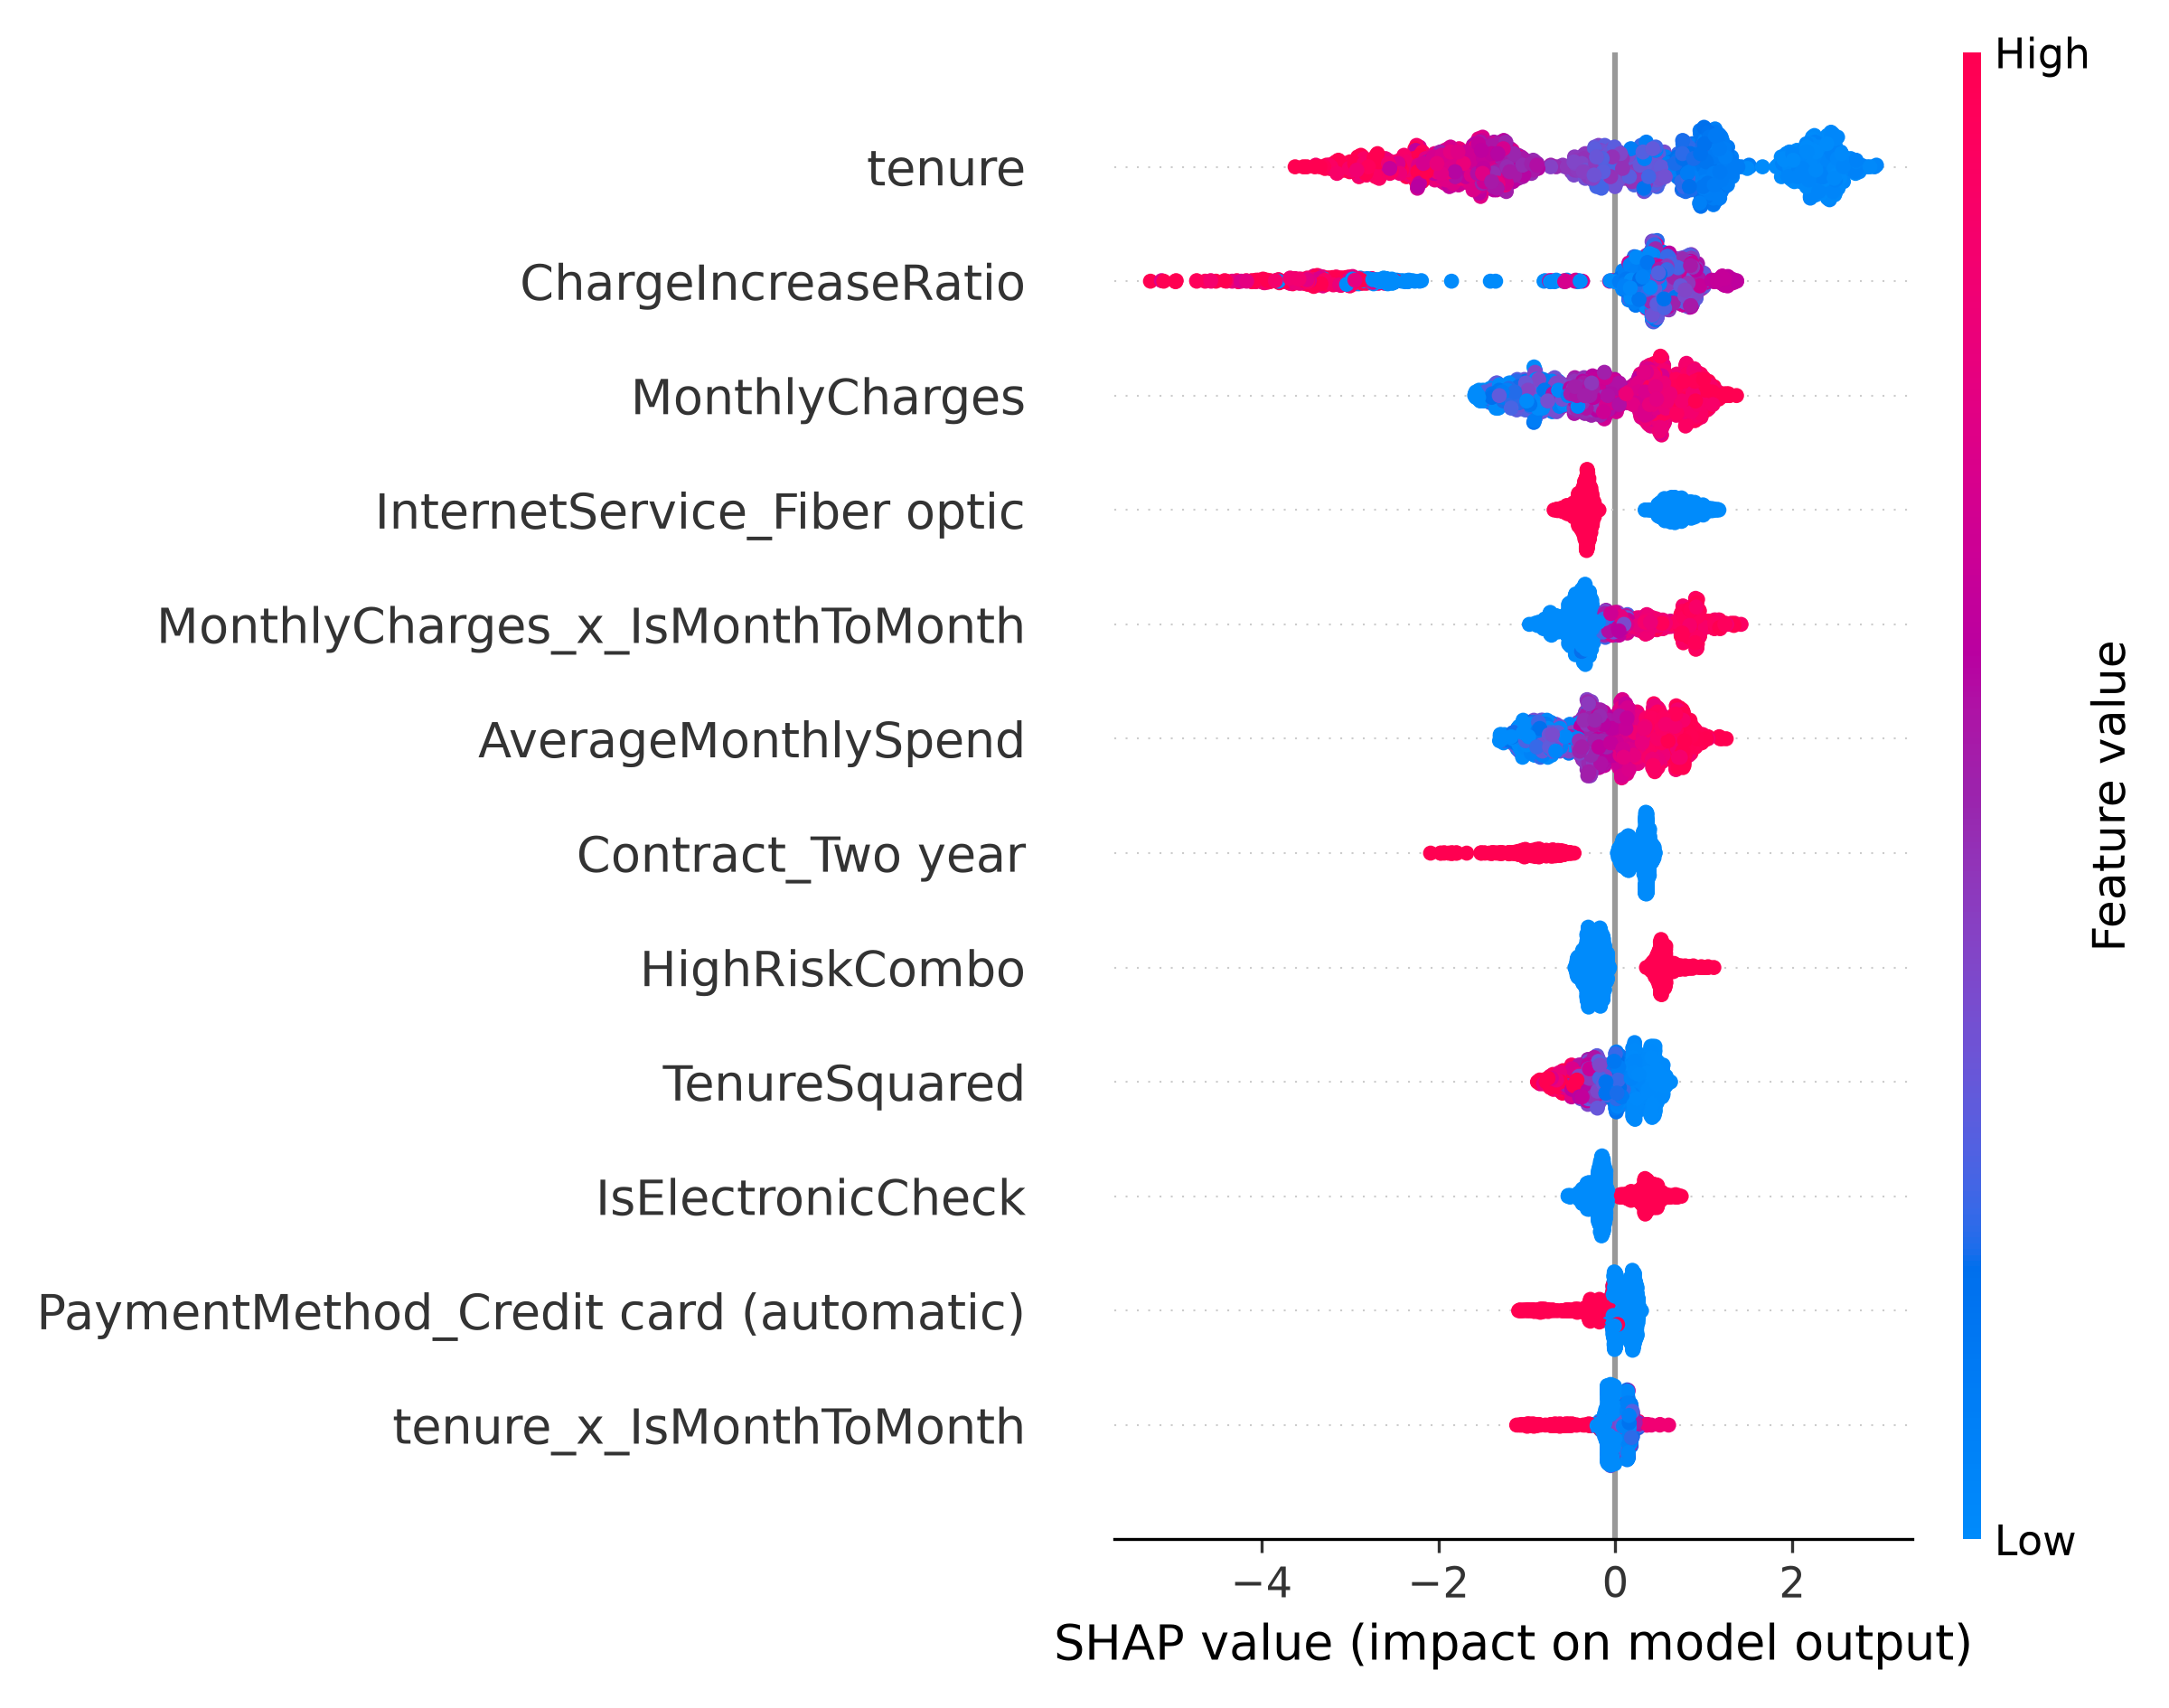
\includegraphics[width=\columnwidth]{shap_summary_beeswarm.png}
\caption{SHAP summary beeswarm plot illustrating directional feature impact.}
\label{fig:shap_beeswarm}
\end{figure}

The empirical ranking reveals the primary drivers of subscriber attrition:
\begin{enumerate}
    \item \textit{Tenure Dynamics:} \texttt{tenure} ranks first (Mean $|\text{SHAP}| = 1.4539$), followed by \texttt{TenureSquared} (0.2917). Low tenure ($<6$ months) strongly elevates churn hazard, while tenure $>24$ months provides robust protective retention.
    \item \textit{Billing Escalation:} \texttt{ChargeIncreaseRatio} ranks second (1.0795), followed by \texttt{MonthlyCharges} (0.6410) and \texttt{AverageMonthlySpend} (0.4769). Escalating bills relative to historic baseline trigger immediate subscriber price sensitivity.
    \item \textit{Service Infrastructure:} \texttt{InternetService\_Fiber optic} (0.5199) demonstrates strong positive churn association, reflecting competitive fiber promotional churning.
    \item \textit{Interaction Effects:} \texttt{MonthlyCharges\_x\_IsMonthToMonth} (0.4880) and \texttt{HighRiskCombo} (0.3345) confirm that high recurring expenditure combined with zero contractual friction compounds defection risk.
\end{enumerate}

\subsection{Quantitative SHAP vs. LIME Concordance Analysis}
To evaluate the widespread assumption that local XAI explainers produce concordant explanations, we conducted an empirical concordance experiment across $N = 200$ test customer instances using identical 27-dimensional feature representations.

\begin{table}[htbp]
\centering
\caption{Quantitative Concordance Between SHAP and LIME ($N=200$ Customers)}
\label{tab:concordance}
\begin{tabular}{lcccc}
\toprule
\textbf{Metric} & \textbf{Mean} & \textbf{Std Dev} & \textbf{Median} & \textbf{Empirical Alignment} \\
\midrule
Spearman Rank Correlation ($\rho$) & 0.2421 & 0.1091 & 0.2444 & Weak-to-moderate \\
Top-3 Feature Set Overlap & 22.83\% & 22.00\% & 33.33\% & Low agreement \\
Top-5 Feature Set Overlap & 38.80\% & 13.80\% & 40.00\% & Moderate divergence \\
\bottomrule
\end{tabular}
\end{table}

As documented in Table \ref{tab:concordance}, the quantitative results demonstrate substantial divergence:
\begin{itemize}
    \item The mean Spearman rank correlation is only **$0.2421 \pm 0.1091$** (median: 0.2444).
    \item Top-3 feature overlap averages only **22.83\%**, indicating that SHAP and LIME identify the same primary risk drivers in less than one in four customer records.
    \item \textbf{Mathematical Root Cause:} TreeSHAP evaluates non-linear feature interactions over the global data manifold satisfying game-theoretic axioms. In contrast, LIME fits a local ridge regression over perturbed Gaussian samples. In the presence of correlated interaction features (\textit{tenure}, \textit{TenureSquared}, \textit{HighRiskCombo}), LIME distributes surrogate weights inconsistently across collinear dimensions, producing ranking discordance.
\end{itemize}
This empirical finding cautions practitioners against visually relying on single-instance LIME plots without statistical validation.

\subsection{Representative Customer Case Studies}
Fig. \ref{fig:local_xai} illustrates dual SHAP and LIME local explanations for a high-risk subscriber, evaluated alongside a low-risk case:

\begin{figure}[htbp]
\centering
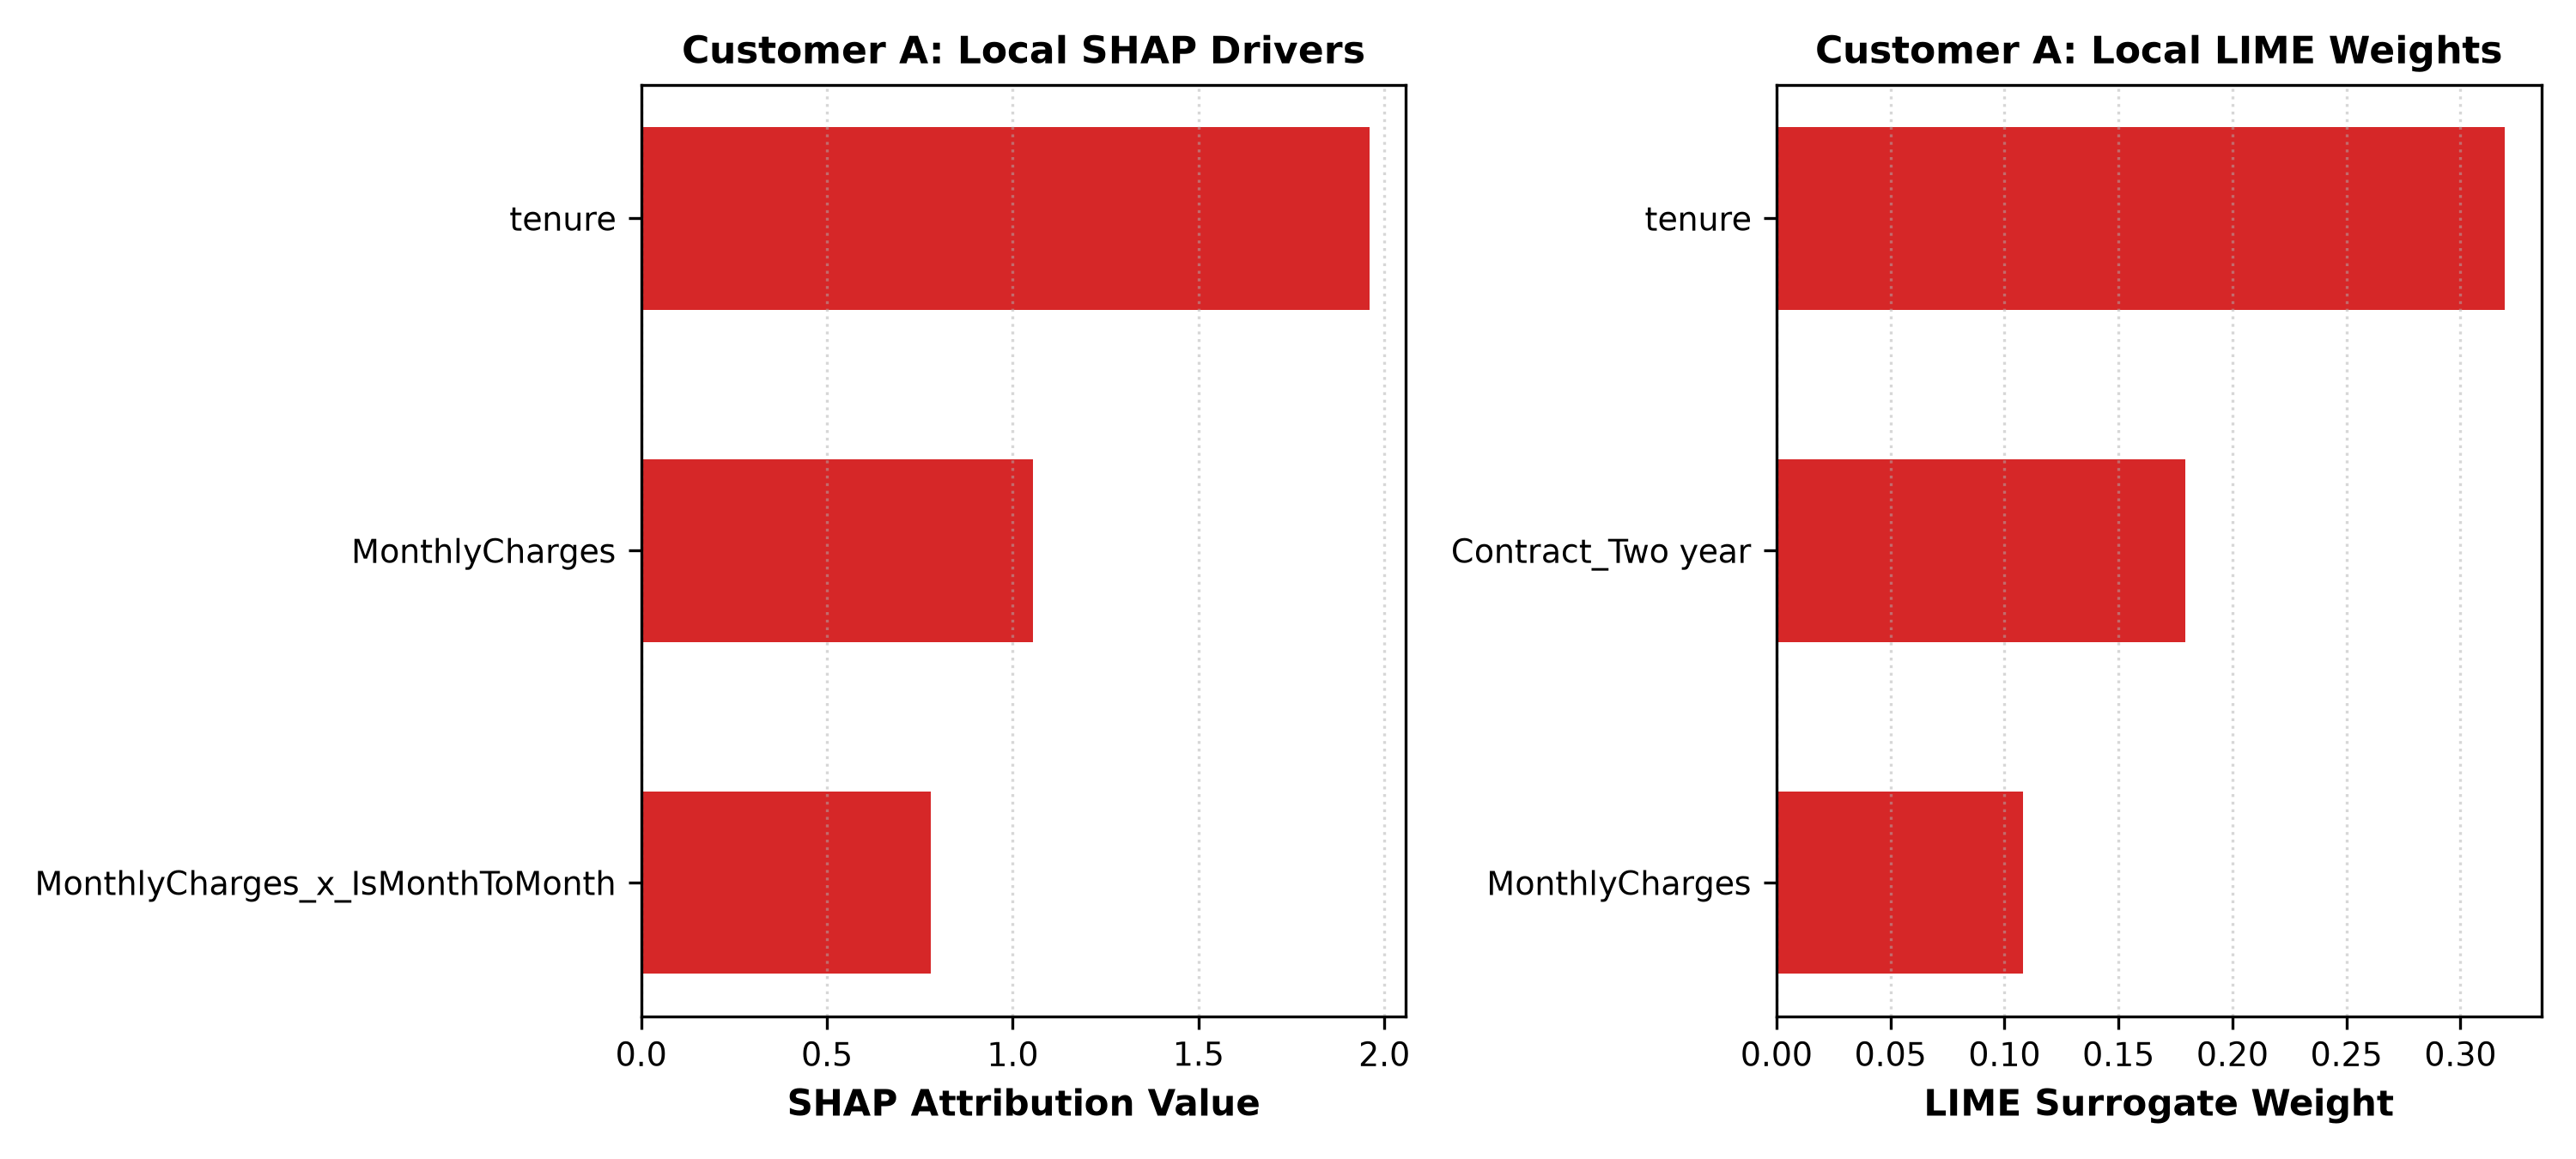
\includegraphics[width=\columnwidth]{local_xai_customer_a.png}
\caption{Side-by-side local SHAP and LIME attributions for Customer A.}
\label{fig:local_xai}
\end{figure}

\begin{itemize}
    \item \textbf{Customer A (High-Risk Defector):} Profile: Tenure = 4 months, Month-to-month contract, Electronic check, MonthlyCharges = $\$101.14$.
    \begin{itemize}
        \item \textit{Predicted Churn Probability:} \textbf{97.89\%} (Class: High Risk at $\tau = 0.26$).
        \item \textit{Top SHAP Factors:} \texttt{tenure} (+1.9602), \texttt{MonthlyCharges} (+1.0551), \texttt{MonthlyCharges\_x\_IsMonthToMonth} (+0.7808).
        \item \textit{Top LIME Factors:} \texttt{tenure <= -0.92} (+0.3195), \texttt{Contract\_Two year <= 0.00} (+0.1793).
        \item \textit{Prescribed Action:} \texttt{Early Lifecycle Onboarding \& Care Outreach} (Priority: \textbf{CRITICAL}).
        \item \textit{State-Awareness Check:} Passed. Customer is uncommitted and early-tenure; intervention targets onboarding vulnerability.
    \end{itemize}
    \item \textbf{Customer B (Loyal Subscriber):} Profile: Tenure = 40 months, Two-year contract, Credit card (automatic), MonthlyCharges = $\$90.53$.
    \begin{itemize}
        \item \textit{Predicted Churn Probability:} \textbf{18.33\%} (Class: Low Risk at $\tau = 0.26$).
        \item \textit{Top SHAP Factors:} \texttt{tenure} (-0.9481, protective), \texttt{Contract\_Two year} (-0.8495, protective), \texttt{MonthlyCharges} (+0.9328, risk factor).
        \item \textit{Prescribed Action:} \texttt{Account Plan \& Rate Optimization Review} (Priority: \textbf{LOW}).
        \item \textit{State-Awareness Check:} \textbf{Passed.} Because Customer B is already on a two-year contract and automatic payment, \textit{Contract Upgrade} and \textit{Autopay Migration} were \textbf{pruned}. Only rate optimization was offered to address the $\$90.53/\text{mo}$ charge.
    \end{itemize}
\end{itemize}

\subsection{Simulated Retention Economics and ROI Analysis}
To evaluate business impact, an empirical simulation was executed on the hold-out test cohort ($N = 1,600$) under explicit operational assumptions ($C_{\text{contact}} = \$50$, retention success probability $r = 0.50$, saved customer value $\text{CLV} = \$500$):
\begin{align}
    \text{Outreach Cost} &= N_{\text{flagged}} \times C_{\text{contact}} = 813 \times \$50 = \$40,650 \\
    \text{Retained Accounts} &= \text{TP} \times r = 770 \times 0.50 = 385.0 \\
    \text{Gross Value Saved} &= 385.0 \times \$500 = \$192,500 \\
    \text{Net Benefit} &= \$192,500 - \$40,650 = \mathbf{\$151,850} \\
    \text{Simulated ROI} &= \frac{\$151,850}{\$40,650} \times 100\% = \mathbf{+373.6\%}
\end{align}
Under these experimental assumptions, deploying the cost-sensitive threshold captures 770 true churners, achieving a projected net financial benefit of $\$151,850$ on 1,600 accounts.

\subsection{End-to-End Latency Benchmarking}
Table \ref{tab:latency} details empirical execution latency across 1,000 prediction runs and 100--200 explanation iterations on CPU hardware.

\begin{table}[htbp]
\centering
\caption{Measured Pipeline Latency Benchmarks (CPU Hardware)}
\label{tab:latency}
\begin{tabular}{lcccc}
\toprule
\textbf{Operation} & \textbf{Batch} & \textbf{Runs} & \textbf{Mean (ms)} & \textbf{P95 (ms)} \\
\midrule
Single-Customer Prediction & 1 & 1,000 & 100.15 & 115.21 \\
Batch Customer Prediction & 100 & 1,000 & 124.41 & 167.30 \\
Local SHAP Explanation & 1 & 200 & \textbf{6.26} & \textbf{8.59} \\
Local LIME Explanation & 1 & 100 & 620.21 & 777.76 \\
\bottomrule
\end{tabular}
\end{table}

The latency benchmarks reveal two critical deployment insights:
\begin{enumerate}
    \item \textbf{Batch Vectorization Efficiency:} Scaling prediction batch size from 1 to 100 increases latency by only 24.2\% (100.15\,ms to 124.41\,ms), yielding an effective throughput of approximately 800 customer evaluations per second.
    \item \textbf{Real-Time Explanations:} Local SHAP executes in **6.26\,ms** (P95: 8.59\,ms), enabling synchronous, interactive rendering in customer care CRM interfaces. Conversely, LIME requires **620.21\,ms** (P95: 777.76\,ms) due to perturbed sampling overhead, restricting LIME to asynchronous background processing.
\end{enumerate}

\section{Discussion}
Our findings demonstrate that high predictive accuracy (94.96\%--94.98\%) is a necessary but insufficient condition for effective enterprise churn mitigation. The critical determinant of operational value is \textbf{decision threshold alignment}: shifting thresholds from symmetric 0.50 cutoffs to cost-optimal operating points ($\tau^* \approx 0.04$--$0.10$) reduces enterprise financial loss by over 50\% across all models.

Furthermore, our quantitative concordance analysis refutes the conventional assumption that local XAI explainers agree out of the box. Because LIME fits local linear approximations that struggle with collinear interaction terms, practitioners should treat tree-based SHAP as the primary interpretability source for automated retention engines.

\section{Limitations}
\begin{itemize}
    \item \textbf{Dataset Scope:} Experiments were conducted exclusively on \texttt{balanced\_telco\_churn.csv} ($N=8,000$). The balanced distribution provides rigorous baseline benchmarking but requires threshold recalibration when deploying to operational populations with natural 2\%--5\% monthly churn prevalences.
    \item \textbf{Simulation Parameters:} Economic ROI values represent analytical simulation estimates based on assumed costs ($C_{\text{FN}}=\$500, C_{\text{FP}}=\$50, r=0.50$), rather than proprietary balance sheets.
\end{itemize}

\section{Future Work}
Future research will investigate: (i) causal uplift modeling to estimate Individual Treatment Effects (ITE) and identify persuadable vs. sleeping-dog subscribers, (ii) dynamic multi-armed bandit retention offer assignment, and (iii) temporal transformer architectures processing continuous Call Detail Records (CDR).

\section{Conclusion}
This paper presented an explainable ensemble learning and operational decision-support framework for telecom churn prediction. Evaluating Random Forest, XGBoost, LightGBM, and Stacking Ensembles under repeated cross-validation established robust predictive baselines ($>94.8\%$ accuracy, $>98.8\%$ ROC-AUC). By integrating cost-sensitive threshold optimization, the framework achieves a 51.2\%--52.8\% reduction in simulated business misclassification costs. Dual XAI analysis revealed key tenure and pricing hazard factors while uncovering significant quantitative divergence between SHAP and LIME ($\rho = 0.2421$). Coupled with a state-aware retention recommendation engine and sub-125\,ms batch inference, the framework bridges the gap between machine learning probability estimation and field-level customer retention.

\bibliographystyle{IEEEtran}
\bibliography{refs}

\end{document}
